\documentclass[a4paper,12pt]{jarticle}
\input ./chap01_preamble.tex
\graphicspath{%
  {../text01-img/}%
}
% !TEX root = ./chap01_01.tex
\begin{document}
\section{今回の授業}
\subsection{目標}
\ \ \ \ ラズベリーパイになれよう

\ \ \ \ 自分のホームページを作れるようになろう

\subsection{授業内容}
%\liststyleLii
\begin{enumerate}
  \item ラズベリーパイとは
  \item ラズベリーパイになれよう(1)
  \item ラズベリーパイになれよう(2)
  \item 自分の紹介ページを作ろう
\end{enumerate}
\subsection{注意点}
%\liststyleLiii
\begin{itemize}
  \item
        授業の合間のきゅうけいでは、遠くのものをながめたりして目を休めましょう
  \item 水分ほきゅうはこまめにしましょう
  \item
        先生が説明中は先生の話を聞きましょう
  \item
        わからないことがあったらTAの先生方にすぐ聞きましょう
\end{itemize}
\subsection{教科書について}
%\liststyleLiv
\begin{itemize}
  \item
        教科書には例題、それに似た問題があります。まずは、例題をよく読みながら試してみましょう。そのあと問題を解きましょう。問題の答えは一番最後のページにあります。
\end{itemize}
\clearpage\subsection{配布物の確認}

\bigskip

%\liststyleLv
\begin{enumerate}
  \item ラズベリーパイ
  \item SDカード(16GB)
  \item でんげんケーブル
  \item HDMIケーブル
  \item GPIOエクステンダー
  \item ヘッドセット
  \item マウス
  \item センサーボード
  \item ウェブカメラ
  \item ディスプレイ(持って帰れません)
\end{enumerate}
\clearpage

\begin{tabular}{cc}
  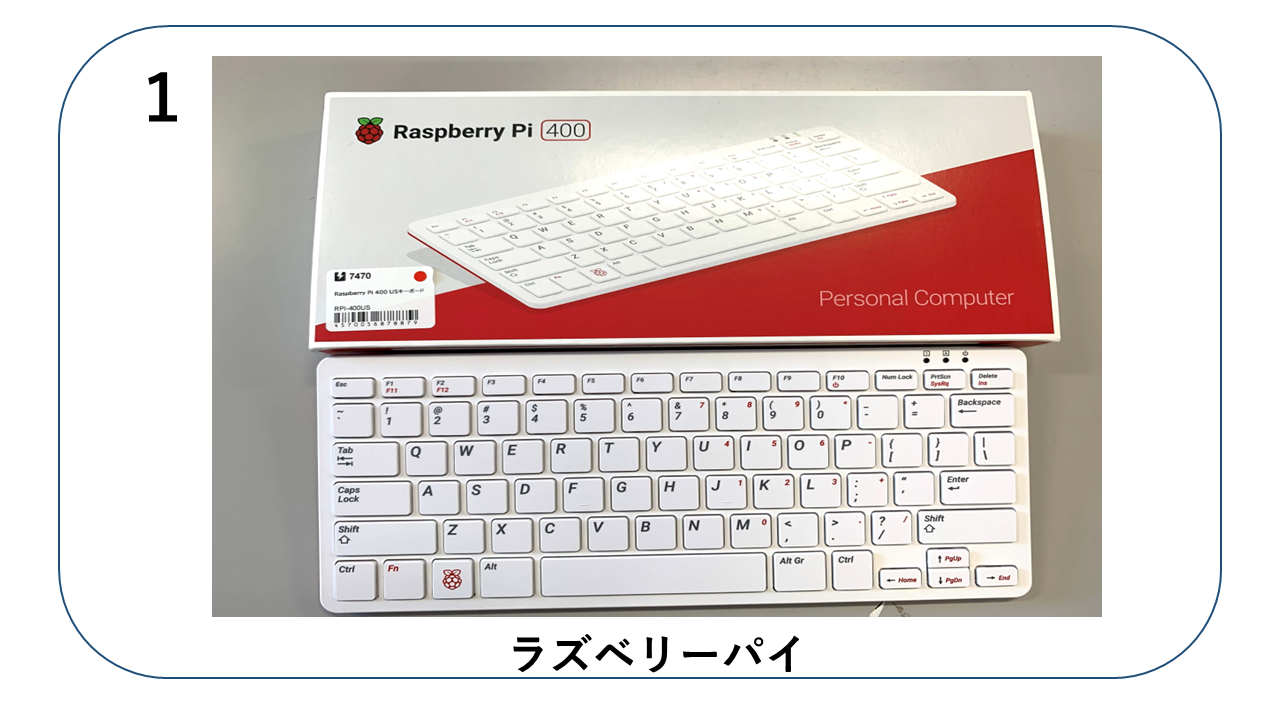
\includegraphics[width=6.488cm,height=4.697cm]{textbook-img009-2023.png}
   &
  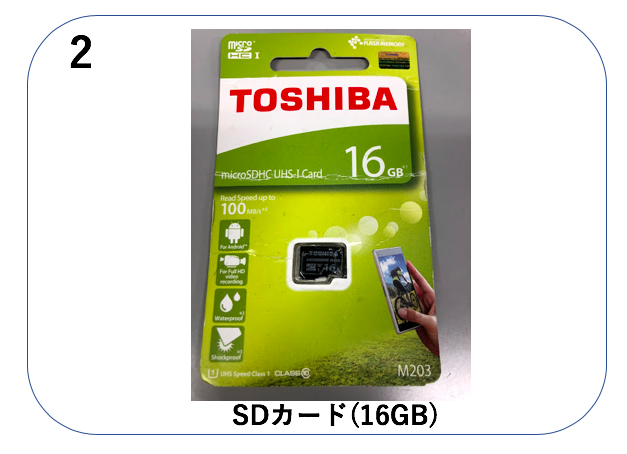
\includegraphics[width=6.488cm,height=4.697cm]{textbook-img010.png} \\

  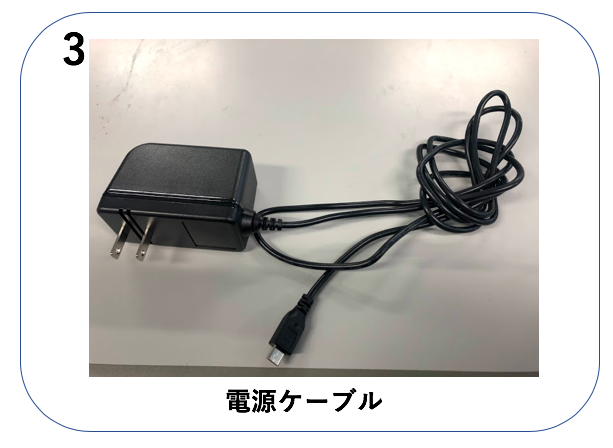
\includegraphics[width=6.488cm,height=4.697cm]{textbook-img007.png}
   &
  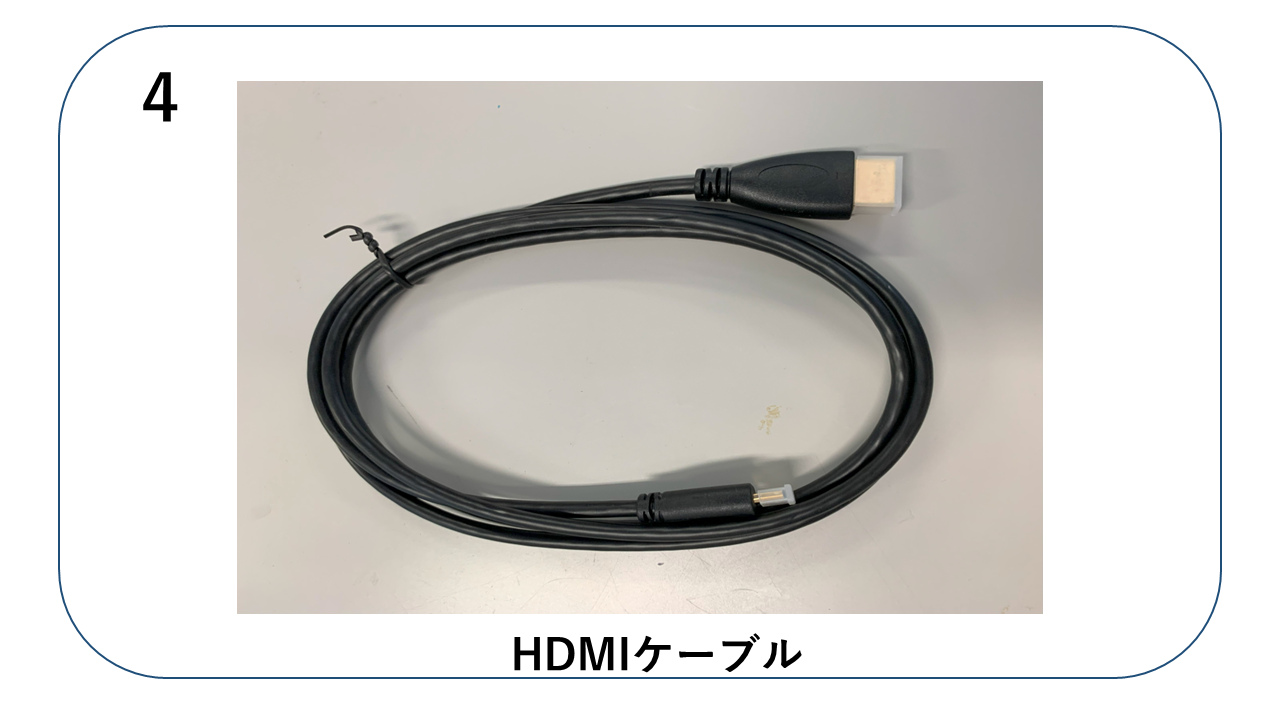
\includegraphics[width=6.488cm,height=4.697cm]{textbook-img008-2023.png} \\

  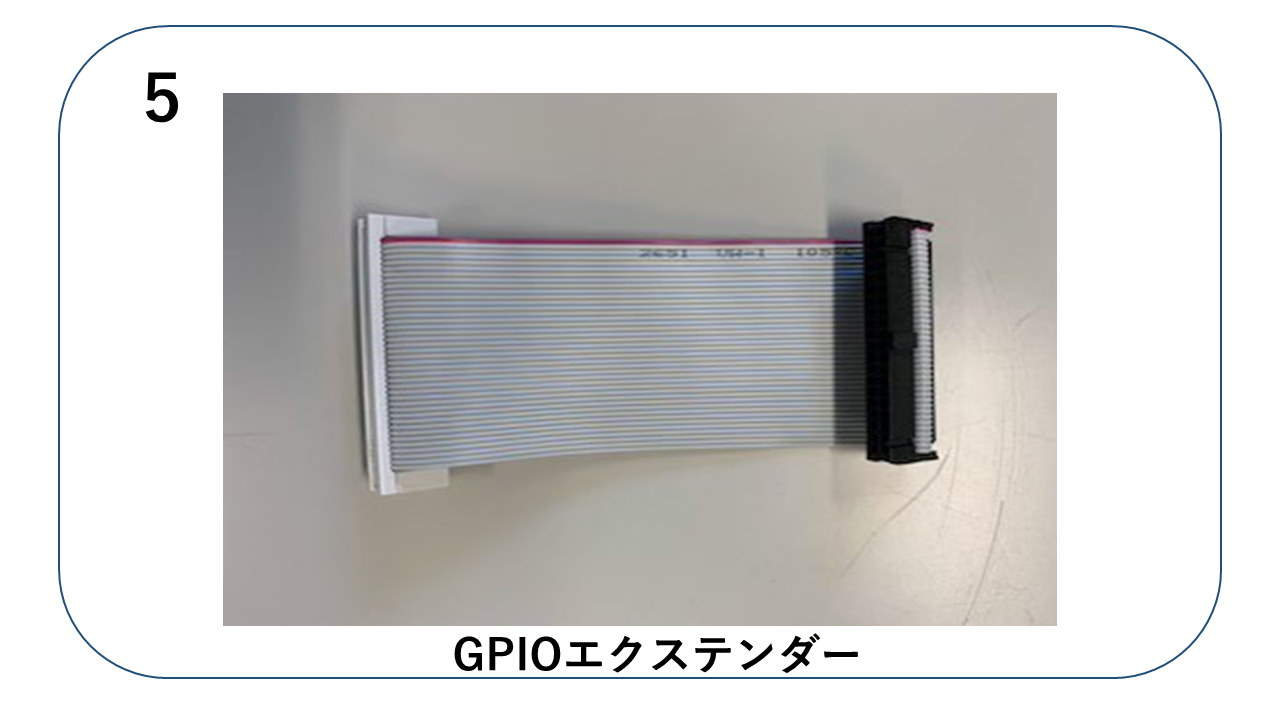
\includegraphics[width=6.488cm,height=4.697cm]{textbook-img005-2023.png}
   &
  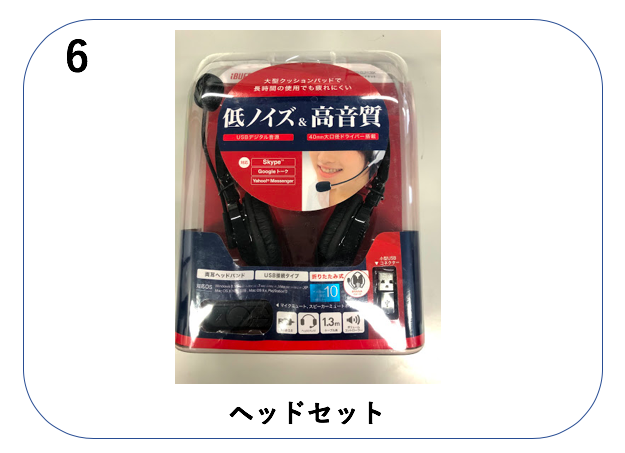
\includegraphics[width=6.488cm,height=4.697cm]{textbook-img006.png} \\

  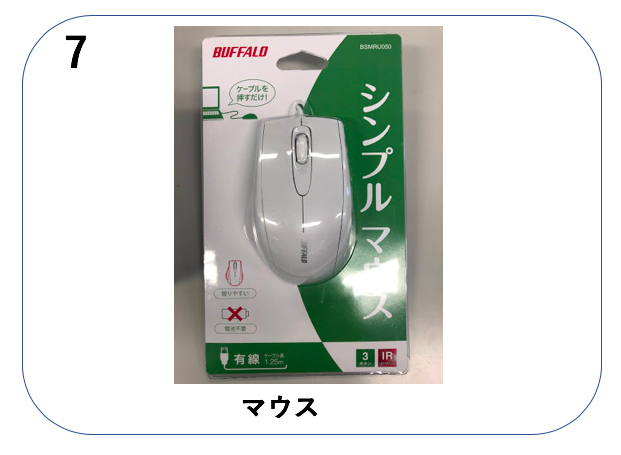
\includegraphics[width=6.488cm,height=4.697cm]{textbook-img003.png}
   &
  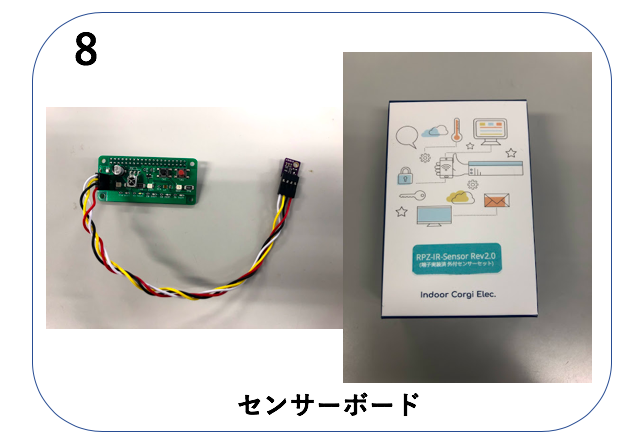
\includegraphics[width=6.488cm,height=4.697cm]{textbook-img004.png} \\

  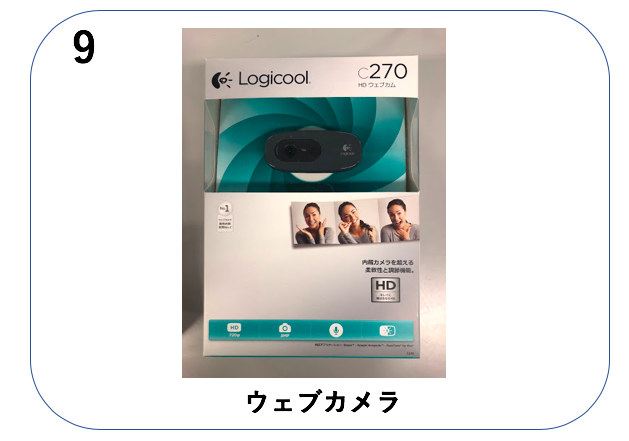
\includegraphics[width=6.488cm,height=4.697cm]{textbook-img002.png}
   &
  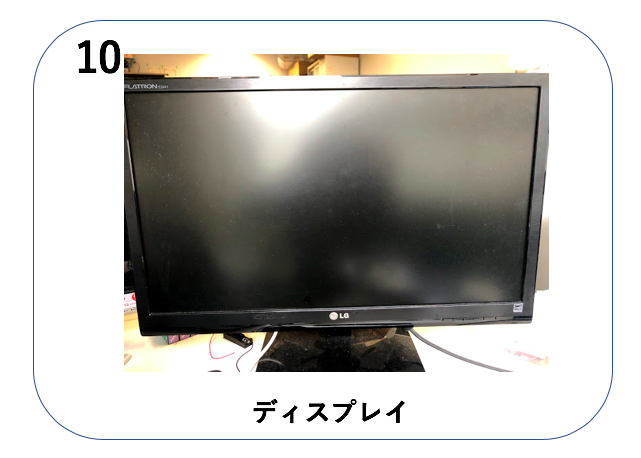
\includegraphics[width=6.488cm,height=4.697cm]{textbook-img001.png} \\
\end{tabular}

%\liststyleLv
\subsection{ラズベリーパイについて}
イギリスのラズベリーパイ財団というグループが開発したコンピュータです。いろいろな種類がありますが、子供IT未来塾ではキーボード一体型タイプのラズベリーパイを使用しています。ラズベリーパイは短くラズパイとも呼ばれています。

\subsection{とくちょう}
%\liststyleLvi
\begin{itemize}
  \item キーボード一体型で、キーボードが必要ない
  \item 普通のパソコンのように使える
  \item (動画再生やゲームもできます)
  \item
        プログラミングのべんきょうに向いている
  \item
        モータやライトをせいぎょできる(目に見えるのでプログラミングを楽しめる)
\end{itemize}
\subsection{ラズベリーパイでできること}
プログラミングを手軽に学ぶことができます。プログラミングをするときにはパソコンが必要

でお金もかかりやりたくてもできないひともいたかもしれません。しかし、ラズベリーパイの

ような小さくて手に入れやすいコンピュータがあれば手軽にプログラミングの学習に取り組む

ことができます。また、ラズベリーパイを使うことでモータやライトなどを動かしたり光らせ

たりすることができます。これらのせいぎょをプログラムで行うことができるので楽しみなが

ら学習を進められます。

\subsection{ラズベリーパイを使うときの注意}
%\liststyleLvii
\begin{itemize}
  \item
        水などぬれているものをラズベリーパイ本体につけないようにしましょう
\end{itemize}
%\liststyleLviii
\begin{itemize}
  \item
        ラズベリーパイをはじめコンピュータなどは熱に弱いのですごく暑い部屋では使わないようにしましょう
\end{itemize}
%\liststyleLix
\begin{itemize}
  \item
        ラズベリーパイなどは静電気によわいので注意しましょう
\end{itemize}
%\liststyleLx
\begin{itemize}
  \item
        ラズベリーパイをらんぼうに扱うのはやめましょう
\end{itemize}


\clearpage

\subsection{ラズベリーパイを準備しよう(手順)}
\ \ ラズベリーパイとマウス等を接続して起動する準備をします。

\begin{figure}[ht]
  \centering
  \begin{minipage}{12.204cm}
    {\upshape
      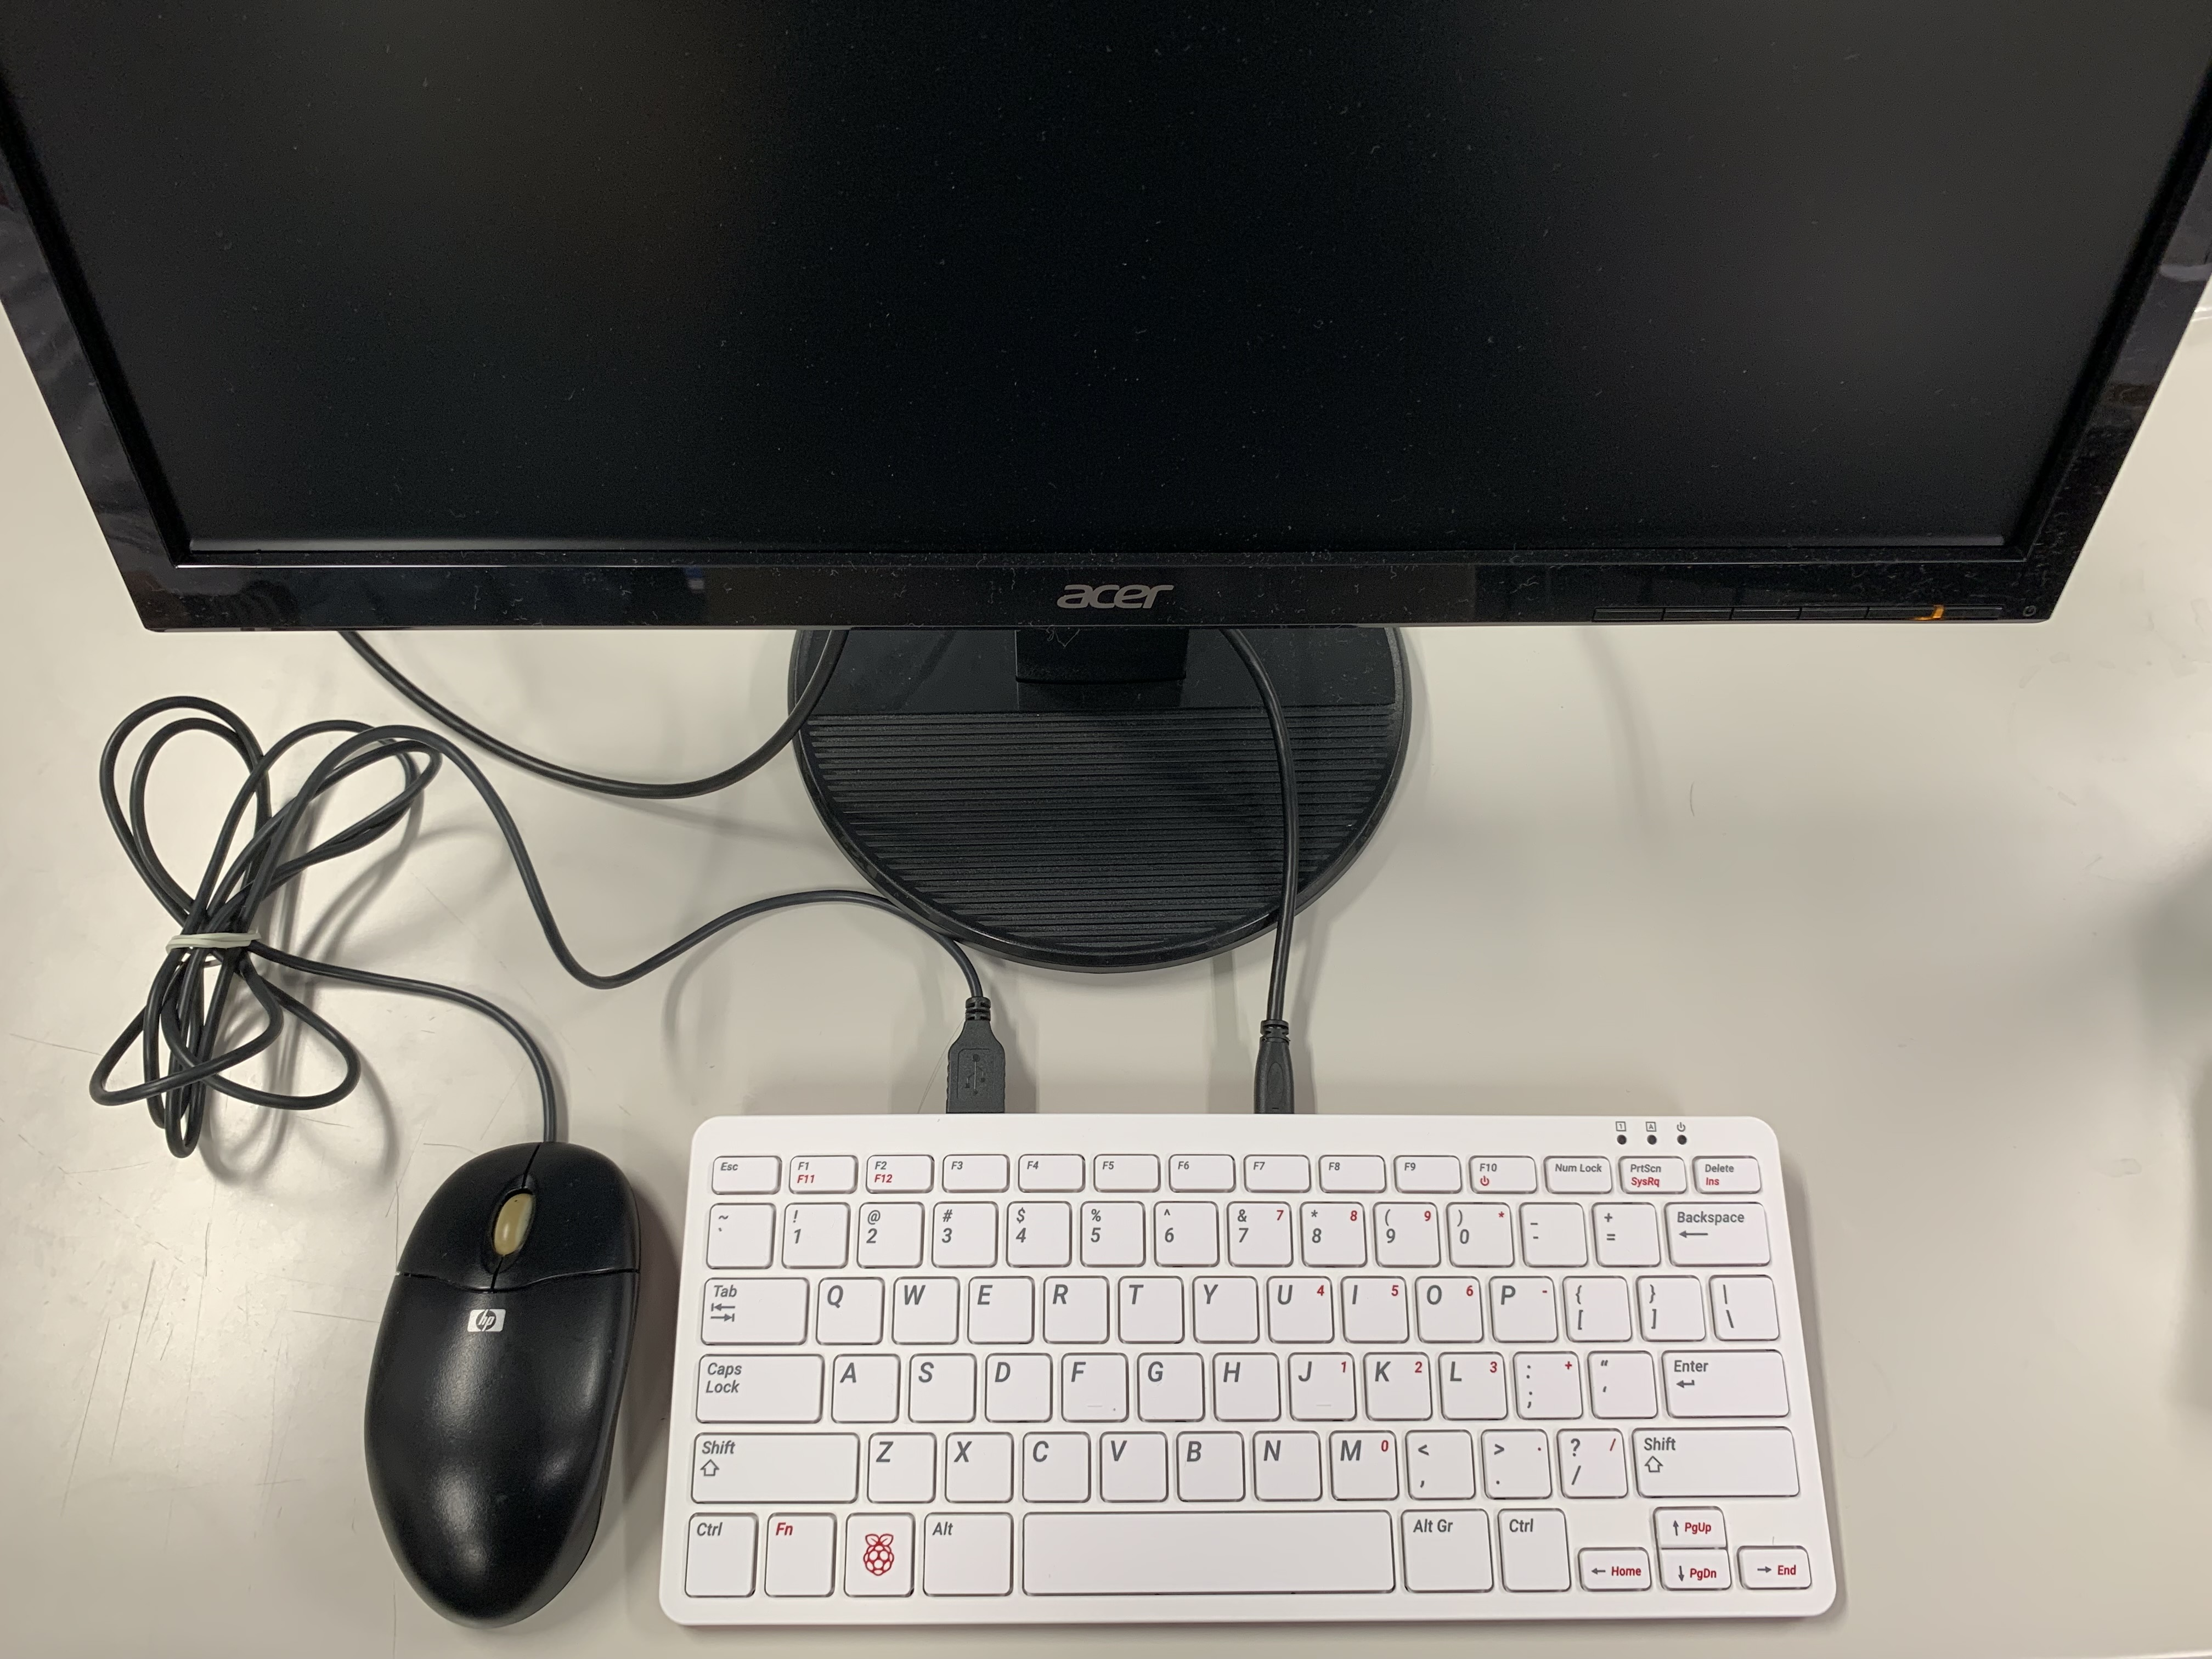
\includegraphics[width=0.6\textwidth]{connections01-2023.jpg}
      \newline
      Figure \stepcounter{Figure}{\theFigure}: 接続の全体図}

  \end{minipage}
\end{figure}

%\liststyleLxii
\begin{enumerate}
  \item ラズベリーパイとモニタをつなぐ

        \begin{itemize}
          \item
                ラズベリーパイとモニタをHDMIケーブルで接続します。右側のHDMIポートを使用してください。Figure~\ref{seq:refFigure1}、Figure~\ref{seq:refFigure2}を参考にしてください。お家でやる場合は、モニタもしくはTVによってはHDMIの差込口の場所が異なる場合があります。説明書等を別途参照してください\textbf{。}


                \begin{figure}[h]
                  \begin{minipage}{0.5\textwidth}
                    {\upshape
                      %[Warning: Image ignored] % Unhandled or unsupported graphics:
                      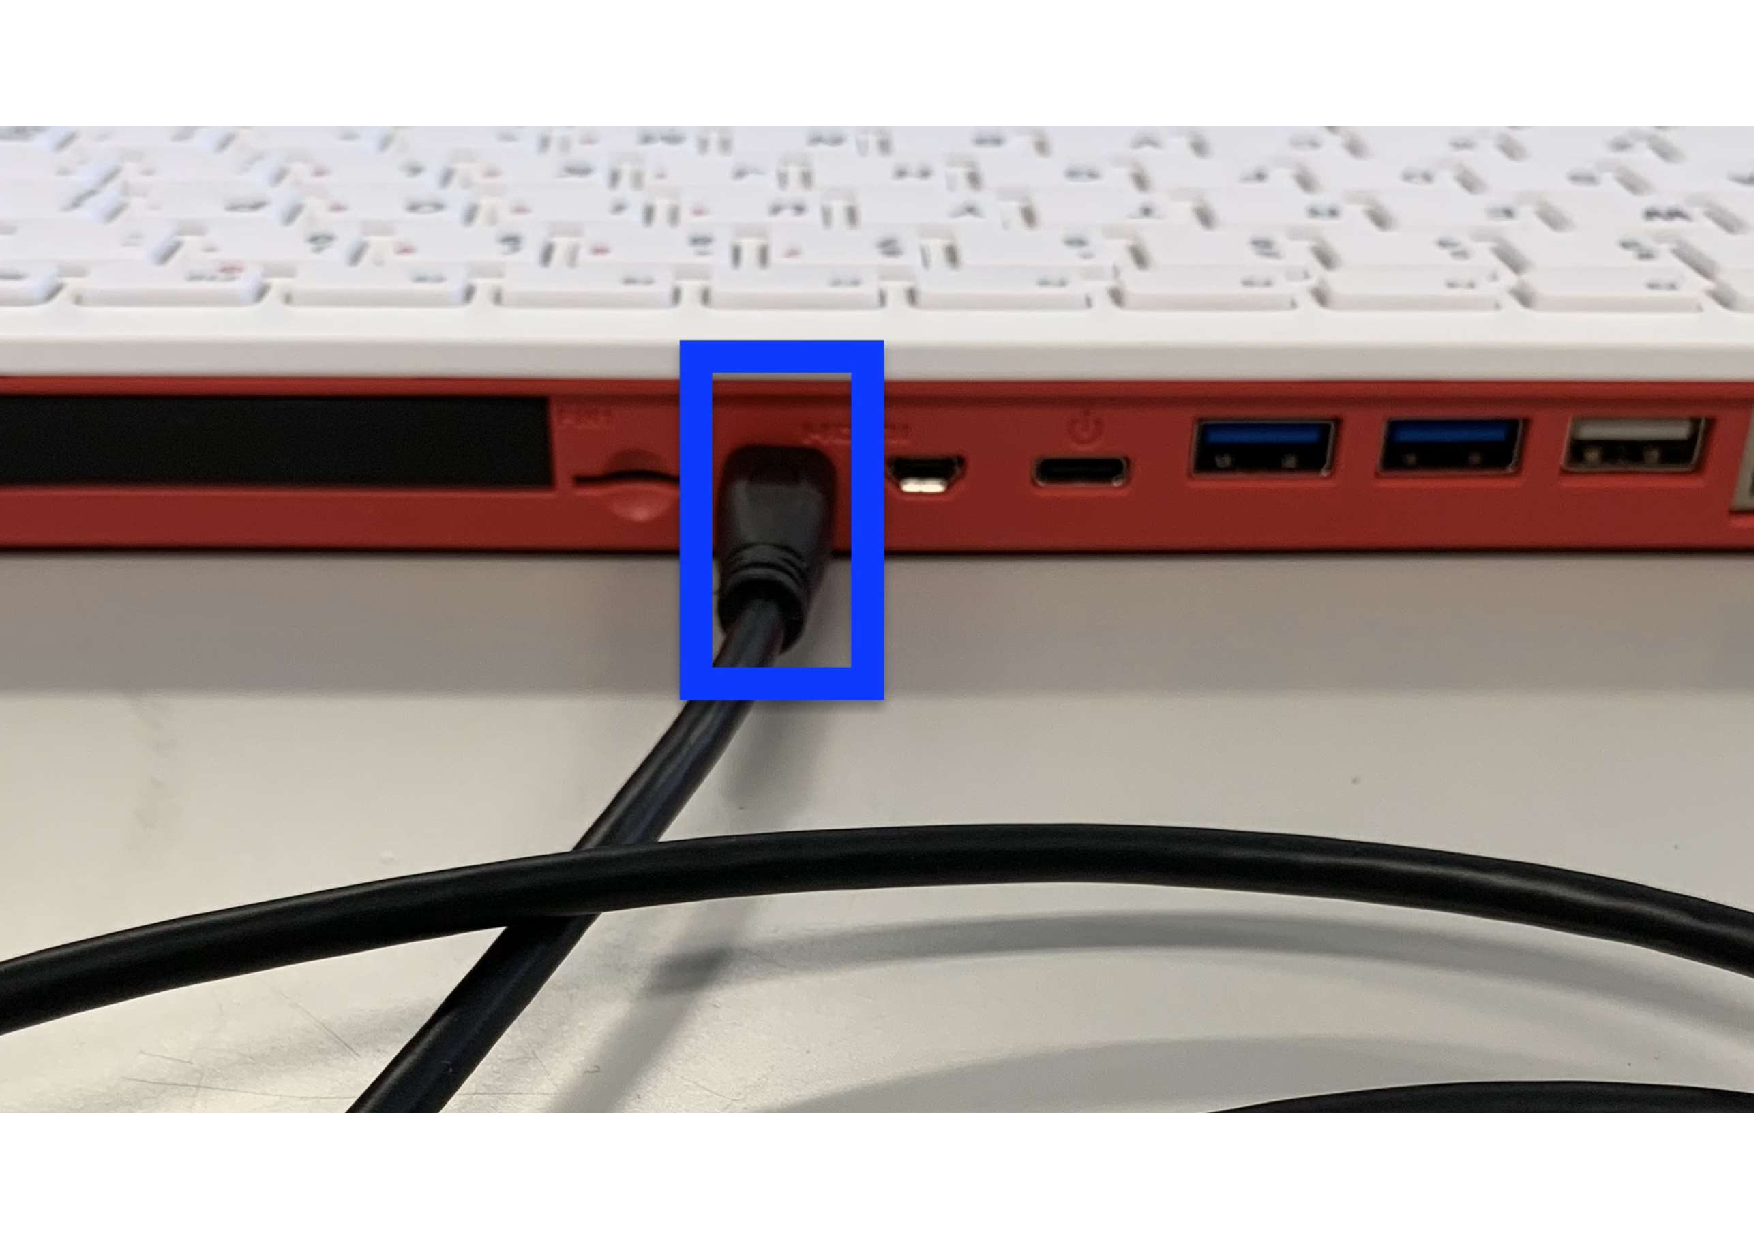
\includegraphics[height=3.471cm]{figure222023.pdf}
                      \newline
                      Figure {\refstepcounter{Figure}\theFigure\label{seq:refFigure1}}:
                      ラズベリーパイHDMI接続}
                  \end{minipage}
                  \begin{minipage}{0.5\textwidth}
                    {\upshape
                      %[Warning: Image ignored] % Unhandled or unsupported graphics:
                      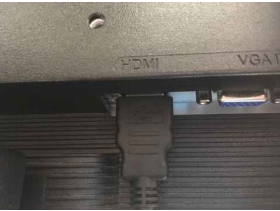
\includegraphics[height=3.471cm]{textbook-img016.png}
                      \newline
                      Figure {\refstepcounter{Figure}\theFigure\label{seq:refFigure2}}:
                      ディスプレイHDMI接続}
                  \end{minipage}
                \end{figure}

        \end{itemize}
  \item マウスをつなぐ

        \begin{itemize}
          \item
                マウスの先をラズベリーパイへ差し込みます。
        \end{itemize}
\end{enumerate}

\begin{figure}[h]
  \begin{minipage}{8.135cm}
    {\upshape
      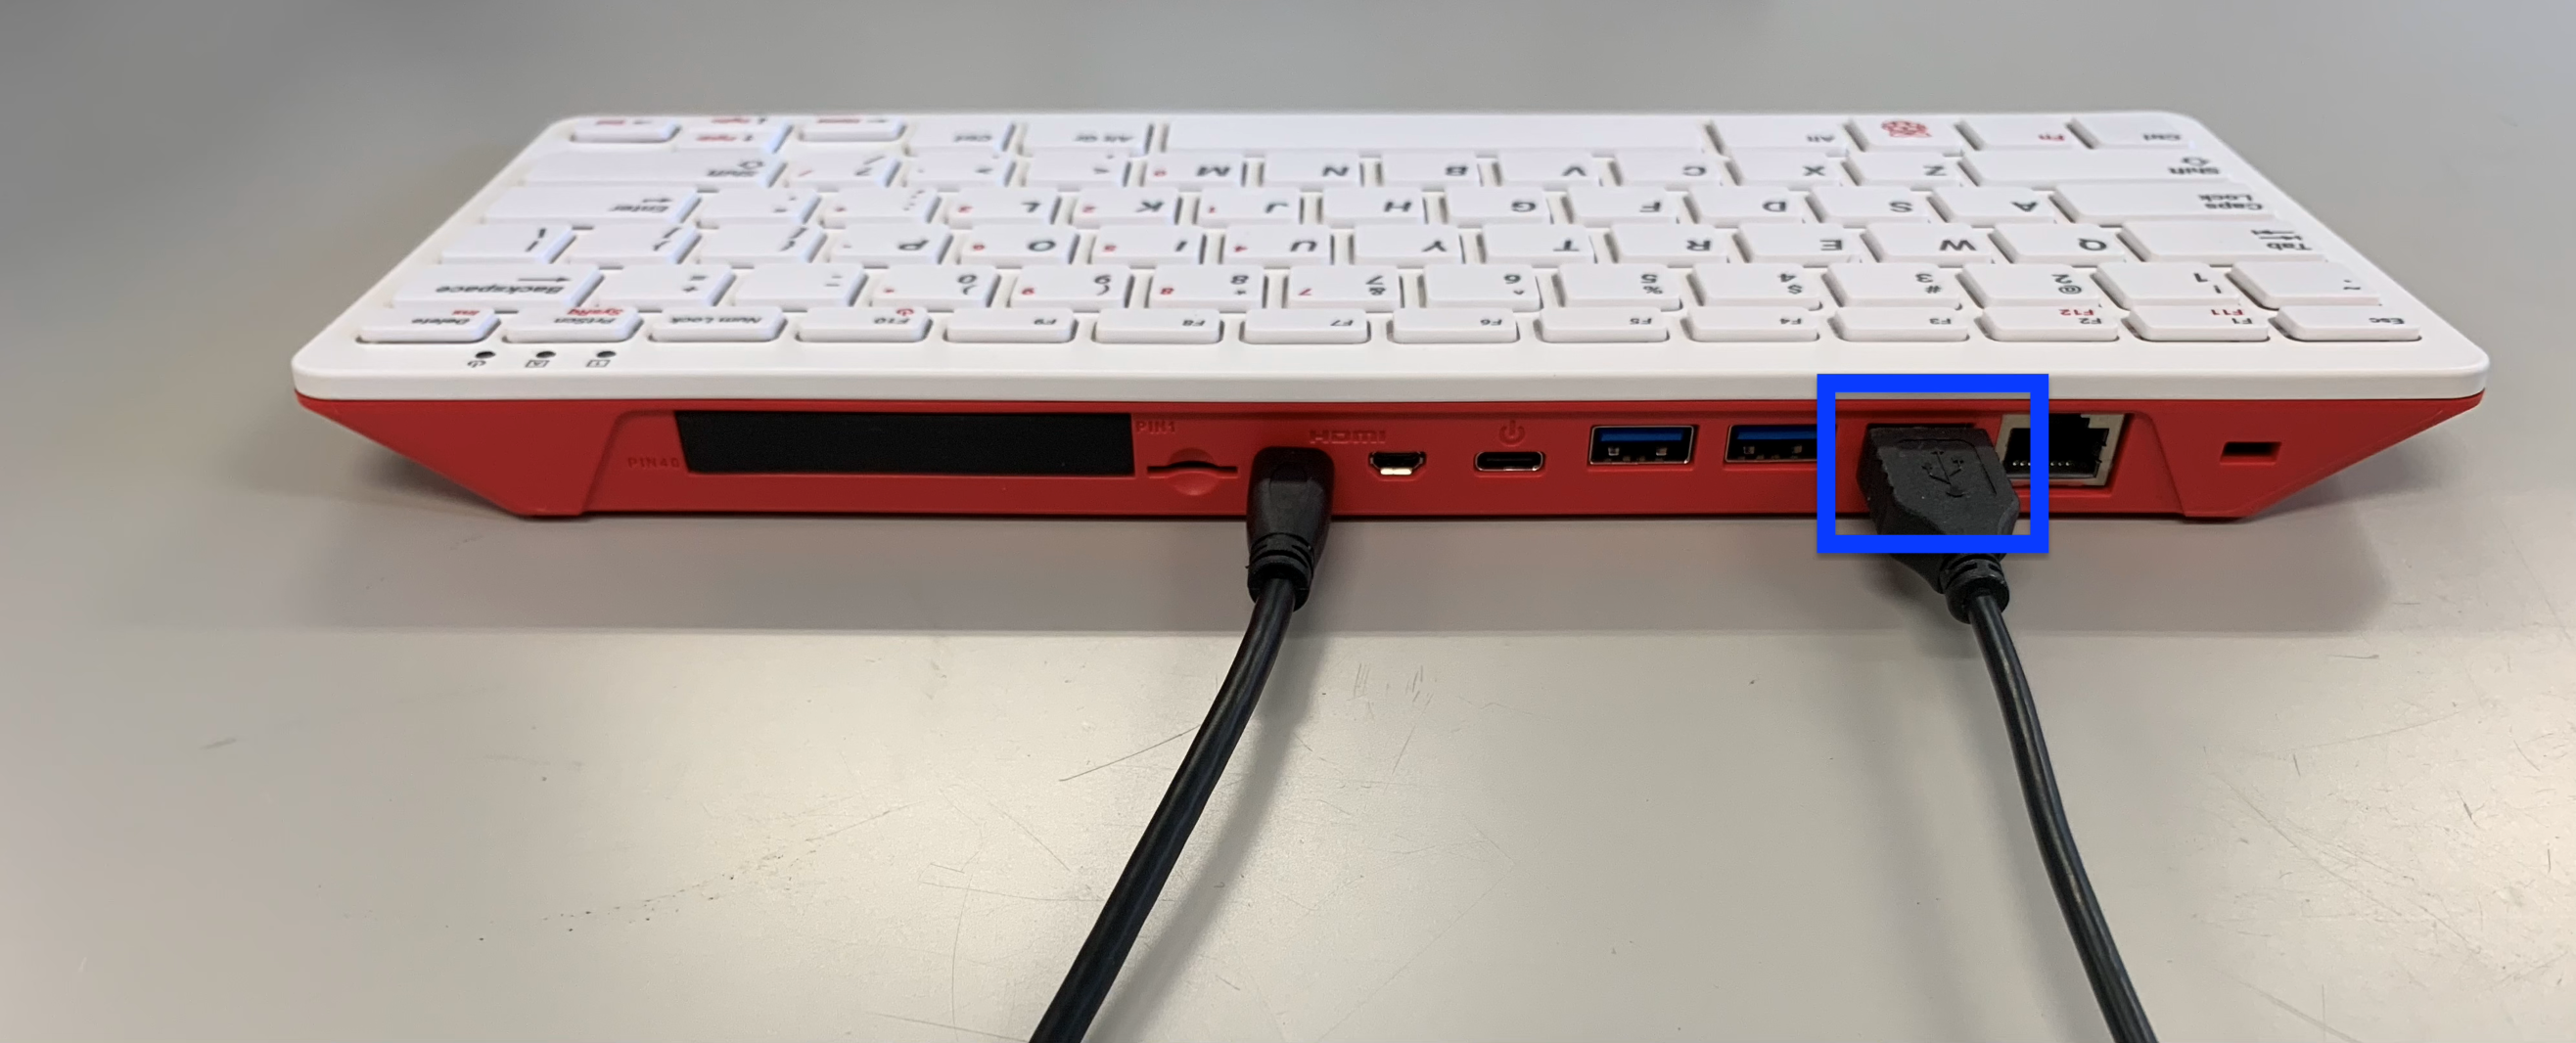
\includegraphics[width=8.135cm]{figure1.10-4.png}
      \newline
      Figure \stepcounter{Figure}{\theFigure}:
      マウス、キーボードの接続}
  \end{minipage}
\end{figure}
%\liststyleLxii
\setcounter{saveenum}{\value{enumi}}
\begin{enumerate}
  \setcounter{enumi}{\value{saveenum}}
  \clearpage
  \item
        microSD(マイクロエスディー)
        カードをいれる

        \begin{itemize}
          \item
                microSDカードをラズベリーパイ本体にさします。小さいのでなくさないように気をつけましょう。

                \begin{figure}[h]
                  \centering
                  \begin{minipage}{6.334cm}
                    {\upshape
                      \includegraphics[width=1\textwidth]{figure1.10-5.png}
                      \newline
                      Figure \stepcounter{Figure}{\theFigure}: microSDカードのさしこみ}
                  \end{minipage}
                \end{figure}

                \bigskip
        \end{itemize}
  \item モニタのでんげんをいれる

        \begin{itemize}
          \item
                次にモニタのコンセントをさします。モニタのみぎはじのボタンをおします。でんげんが入ると青色にてんとうします。お家でやるときはでんげんのいれた後、入力きりかえが必要となる場合がありますので、説明書等を別途参照してください。


                \begin{figure}[h]
                  \centering
                  \begin{minipage}{6.172cm}
                    {\upshape
                      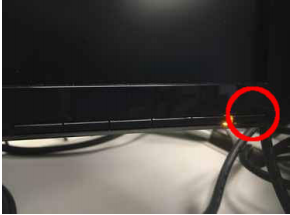
\includegraphics[width=6.318cm,height=4.685cm]{textbook-img019.png}
                      \newline
                      Figure \stepcounter{Figure}{\theFigure}:
                      モニタでんげんボタンの位置}
                  \end{minipage}
                \end{figure}
        \end{itemize}
  \item ラズベリーパイのでんげんをいれる

        \begin{itemize}
          \item
                最後にラズベリーパイのでんげんをいれます。Figure~\ref{seq:refFigure6}のようにラズベリーパイにでんげんケーブルをさしてコンセントへ接続します。緑色のランプがついてディスプレイにラズベリーが表示がされますFigure~\ref{seq:refFigure7}。
        \end{itemize}
        \begin{figure}
          \centering
          \begin{minipage}{0.4\textwidth}
            {\upshape
              \includegraphics[width=.9\linewidth]{textbook-img020-2023.png}
              \newline
              Figure {\refstepcounter{Figure}\theFigure\label{seq:refFigure6}}:
              ラズベリーパイでんげん接続}
          \end{minipage}
          \begin{minipage}{0.4\textwidth}
            {\upshape
              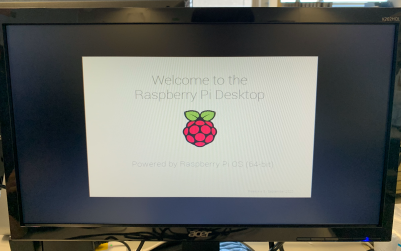
\includegraphics[width=.9\linewidth]{textbook-img0212023.png}
              \newline
              Figure {\refstepcounter{Figure}\theFigure\label{seq:refFigure7}}:
              ラズベリーパイ起動中}
            \end{minipage}
          \end{figure}
          
\clearpage        
\end{enumerate}
\begin{enumerate}

  \subsection{セットアップをしよう}
  \item 定住国を設定して言語とタイムゾーンを決定しよう
        \begin{itemize}
          \item
                raspberry pi 400 が起動すると,このようなFigure~\ref{seq:refFigure8}セットアップの開始画面になります。この画面ではそのままNextのボタンを押して次に進みます。
        \end{itemize} 
        \begin{figure}[h]
          \centering
          \begin{minipage}{5.222cm}
          {\upshape
            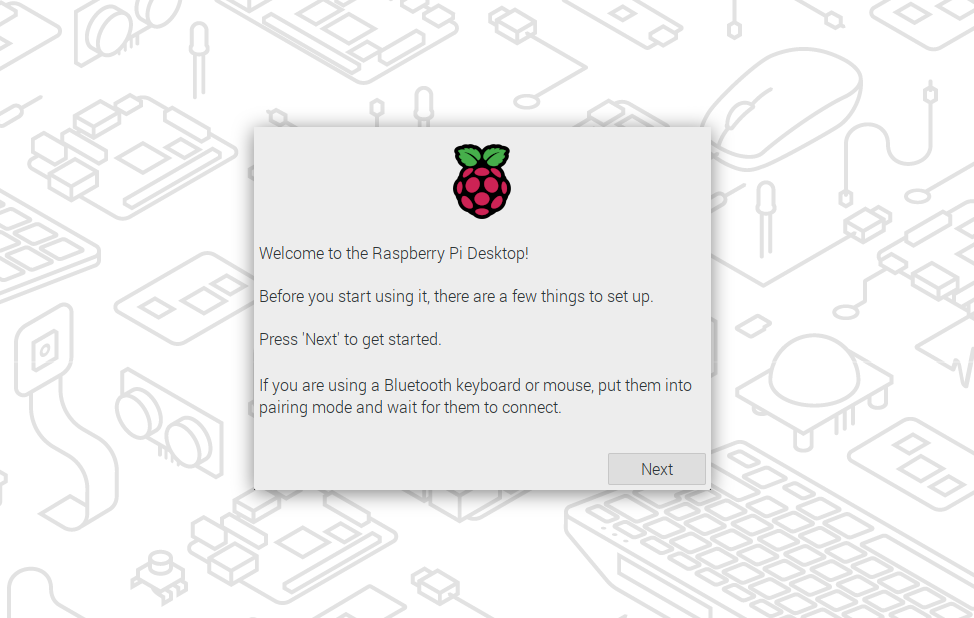
\includegraphics[width=8.613cm]{sw_image01.png}
            \newline
            Figure {\refstepcounter{Figure}\theFigure\label{seq:refFigure8}}:
            起動後画面
          }
        \end{minipage}
        \end{figure}

        \begin{itemize}
          \item
              次の画面ではFigure~\ref{seq:refFigure9}のように自分の住んでいる地域(タイムゾーン)を設定することで言語や時間を決定することができます。今回は皆さん日本に住んでいると思うのでcountryの行をクリックするとFigure~\ref{seq:refFigure10}のように様々な国の名前が表示されるのでその中からJapanを選択してください。そうすると他のLanguage, Timezoneの項目がjapanese,Tokyoになります。これらはそれぞれ言語とタイムゾーンを表しています。それぞれJapan,japanese, Tokyoになっているのを確認できたらNextボタンを押します。※注意: 次の画面に移動したら指示があるまでしばらく待機していてください。
            
              \begin{figure}[h]
                \centering
                \begin{minipage}{5.228cm}
                  {\upshape
                    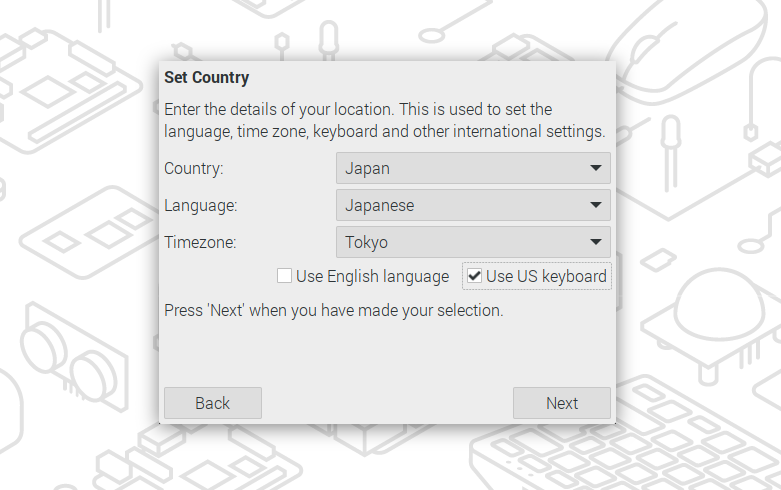
\includegraphics[width=7.000cm,]{sw_image02.png}
                    \newline
                    Figure {\refstepcounter{Figure}\theFigure\label{seq:refFigure9}}:
                    タイムゾーン画面}
                \end{minipage} 
                \centering
                \begin{minipage}{4.228cm}
                  {\upshape
                    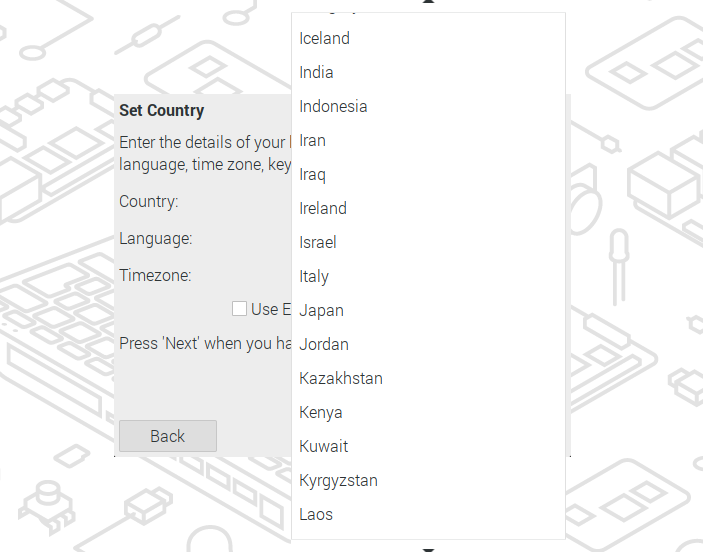
\includegraphics[width=7.000cm]{sw_image03-2.png}
                    \newline
                    Figure {\refstepcounter{Figure}\theFigure\label{seq:refFigure10}}:
                    選択画面}
                \end{minipage}
              \end{figure}    
        \end{itemize}   
        \clearpage 
        \item
        パスワードの重要性について知ろう
        \begin{itemize}
          \item
              IDとパスワードは、パソコンなどの情報機器や、インターネット上のサービスを利用する際に、許可された者であるかを識別し、本人を確認するための重要な情報です。 利用者の範囲が制限されている情報機器やインターネットサービスに、IDとパスワードを入力して、その機器やサービスを利用できる状態にするためのものです。
              \begin{figure}[h]
                \centering
                \begin{minipage}{5.228cm}
                  {\upshape
                    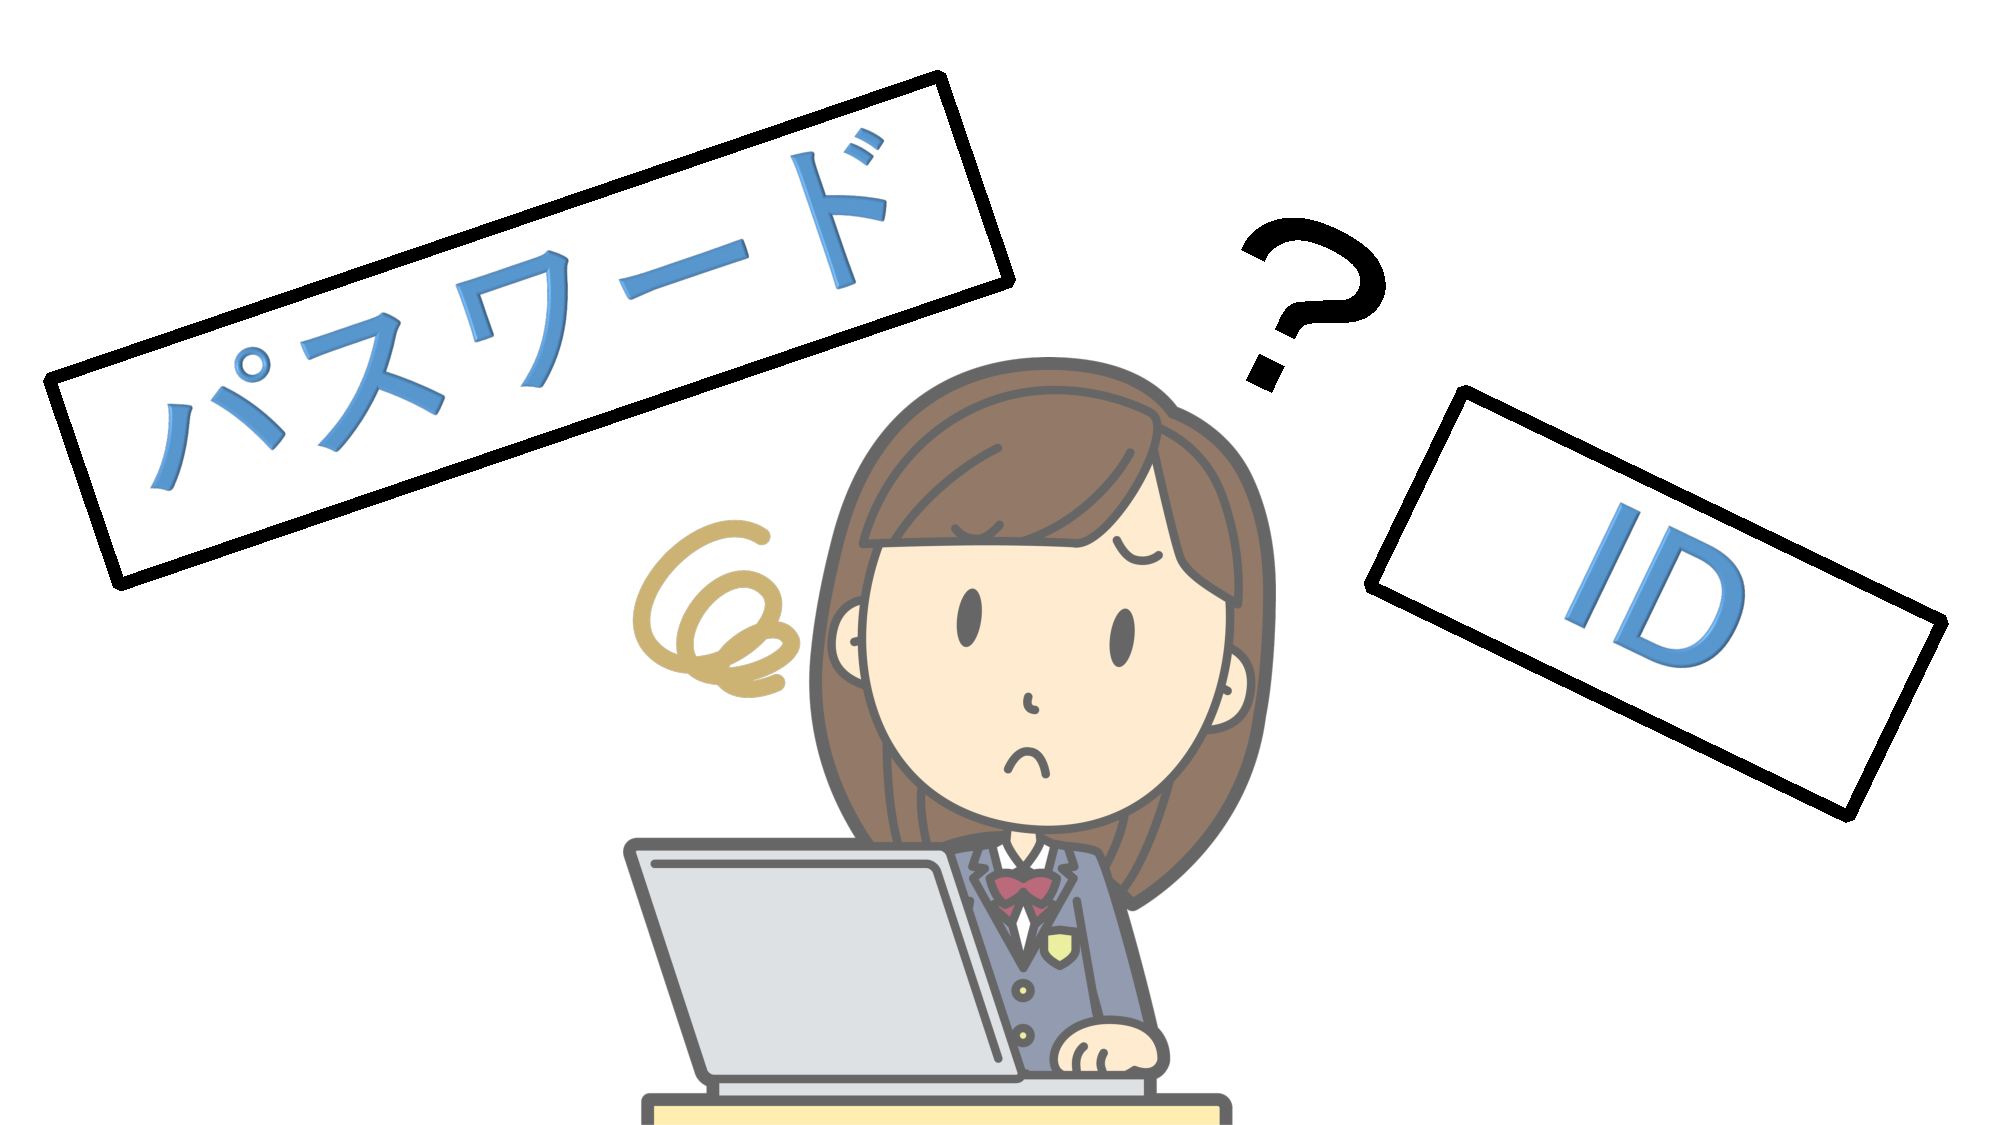
\includegraphics[width=7.000cm]{pswd_image_imp6.pdf}
                    \newline
                    Figure {\refstepcounter{Figure}\theFigure\label{seq:refFigure21}}:
                    ID,パスワード}
                \end{minipage}
              \end{figure}
              \item
              他人に自分のユーザーアカウントを使用されてしまうと、本来は使用権限が与えられていないユーザーがネットワークに接続できるようになったり、データベースから不正に情報を抜き出したりすることができるようになります。
              \begin{figure}[h]
                \centering
                  \begin{minipage}{5.228cm}
                    {\upshape
                      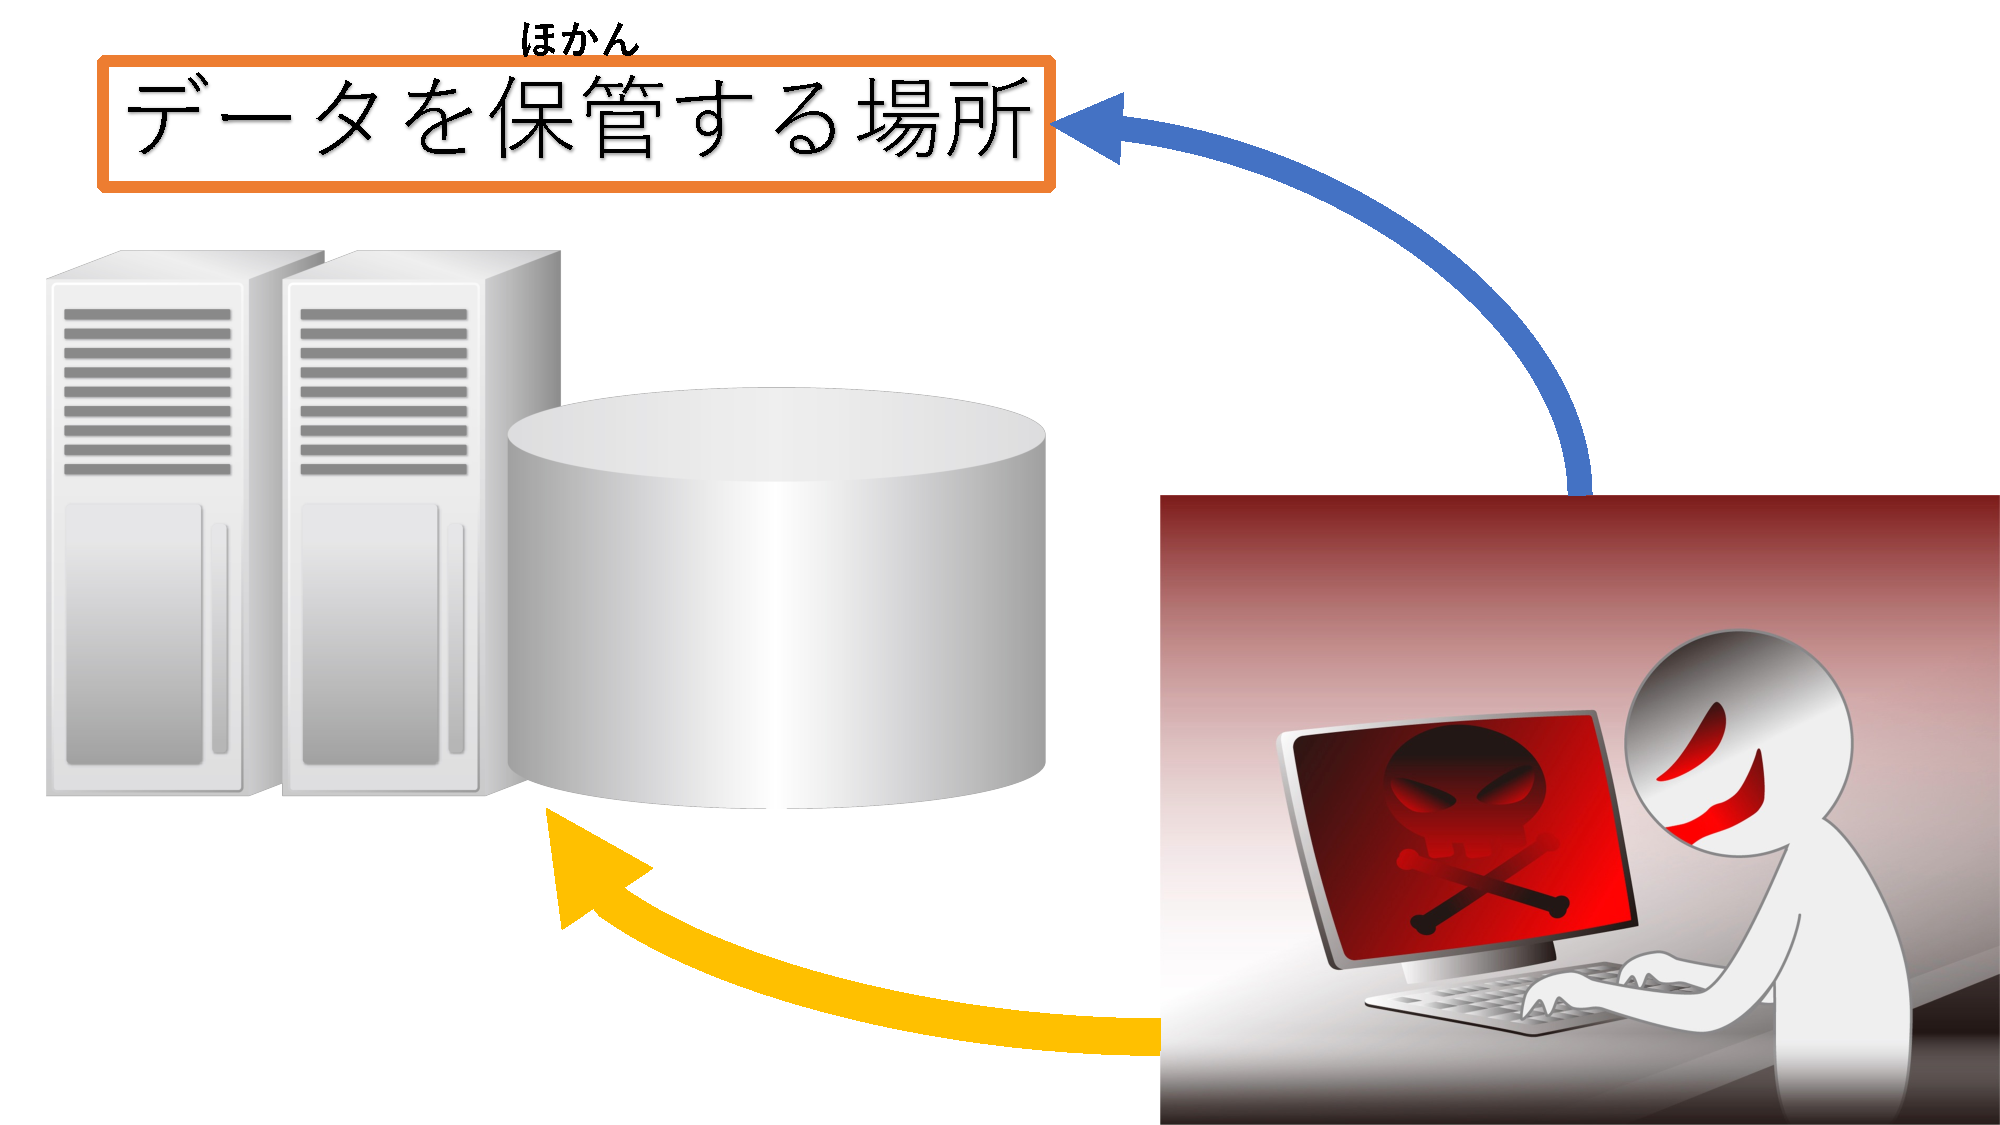
\includegraphics[width=7.000cm]{pswd_image_imp5.pdf}
                      \newline
                      Figure {\refstepcounter{Figure}\theFigure\label{seq:refFigure22}}:
                      不正アクセス}
                  \end{minipage}
                \end{figure}
              \item
              このようななりすましによるハッキングを防止するためには、ひとりひとりのユーザーがパスワードを厳重に管理しなければなりません。
              \begin{figure}[h]
              \centering
                \begin{minipage}{5.228cm}
                  {\upshape
                    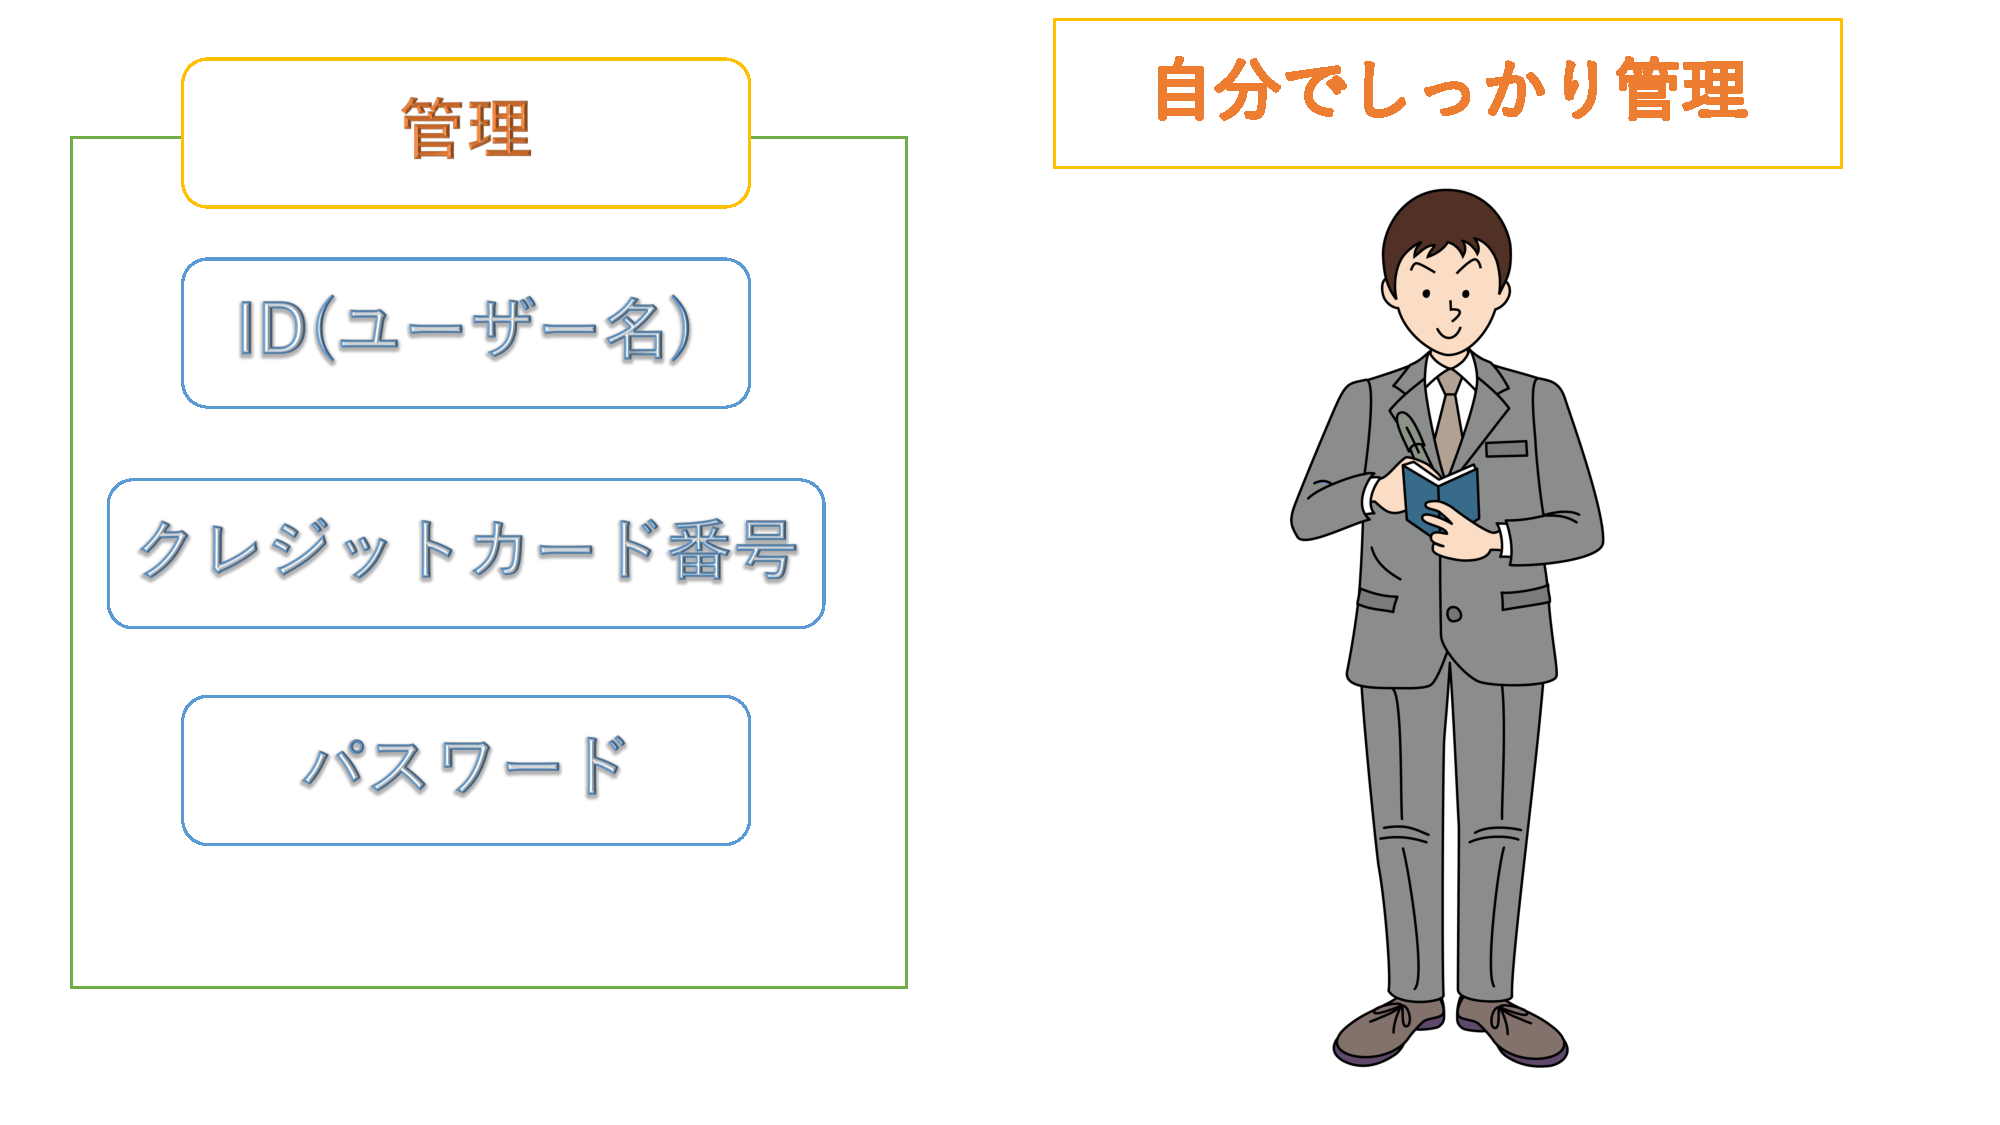
\includegraphics[width=7.000cm]{pswd_image_imp3.pdf}
                    \newline
                    Figure {\refstepcounter{Figure}\theFigure\label{seq:refFigure23}}:
                    パスワード管理}
                \end{minipage}
              \end{figure}
              
              
          \end{itemize}

        
        \clearpage
        \begin{itemize}
        \item
        パスワードをきちんと管理することは、ひとりのユーザーを守るだけでなく、企業や組織全体の情報セキュリティ確保のために大変重要なことです。パスワードの大切さについて再確認しましょう。
        \begin{figure}[h]
          \centering
          \begin{minipage}{5.228cm}
            {\upshape
              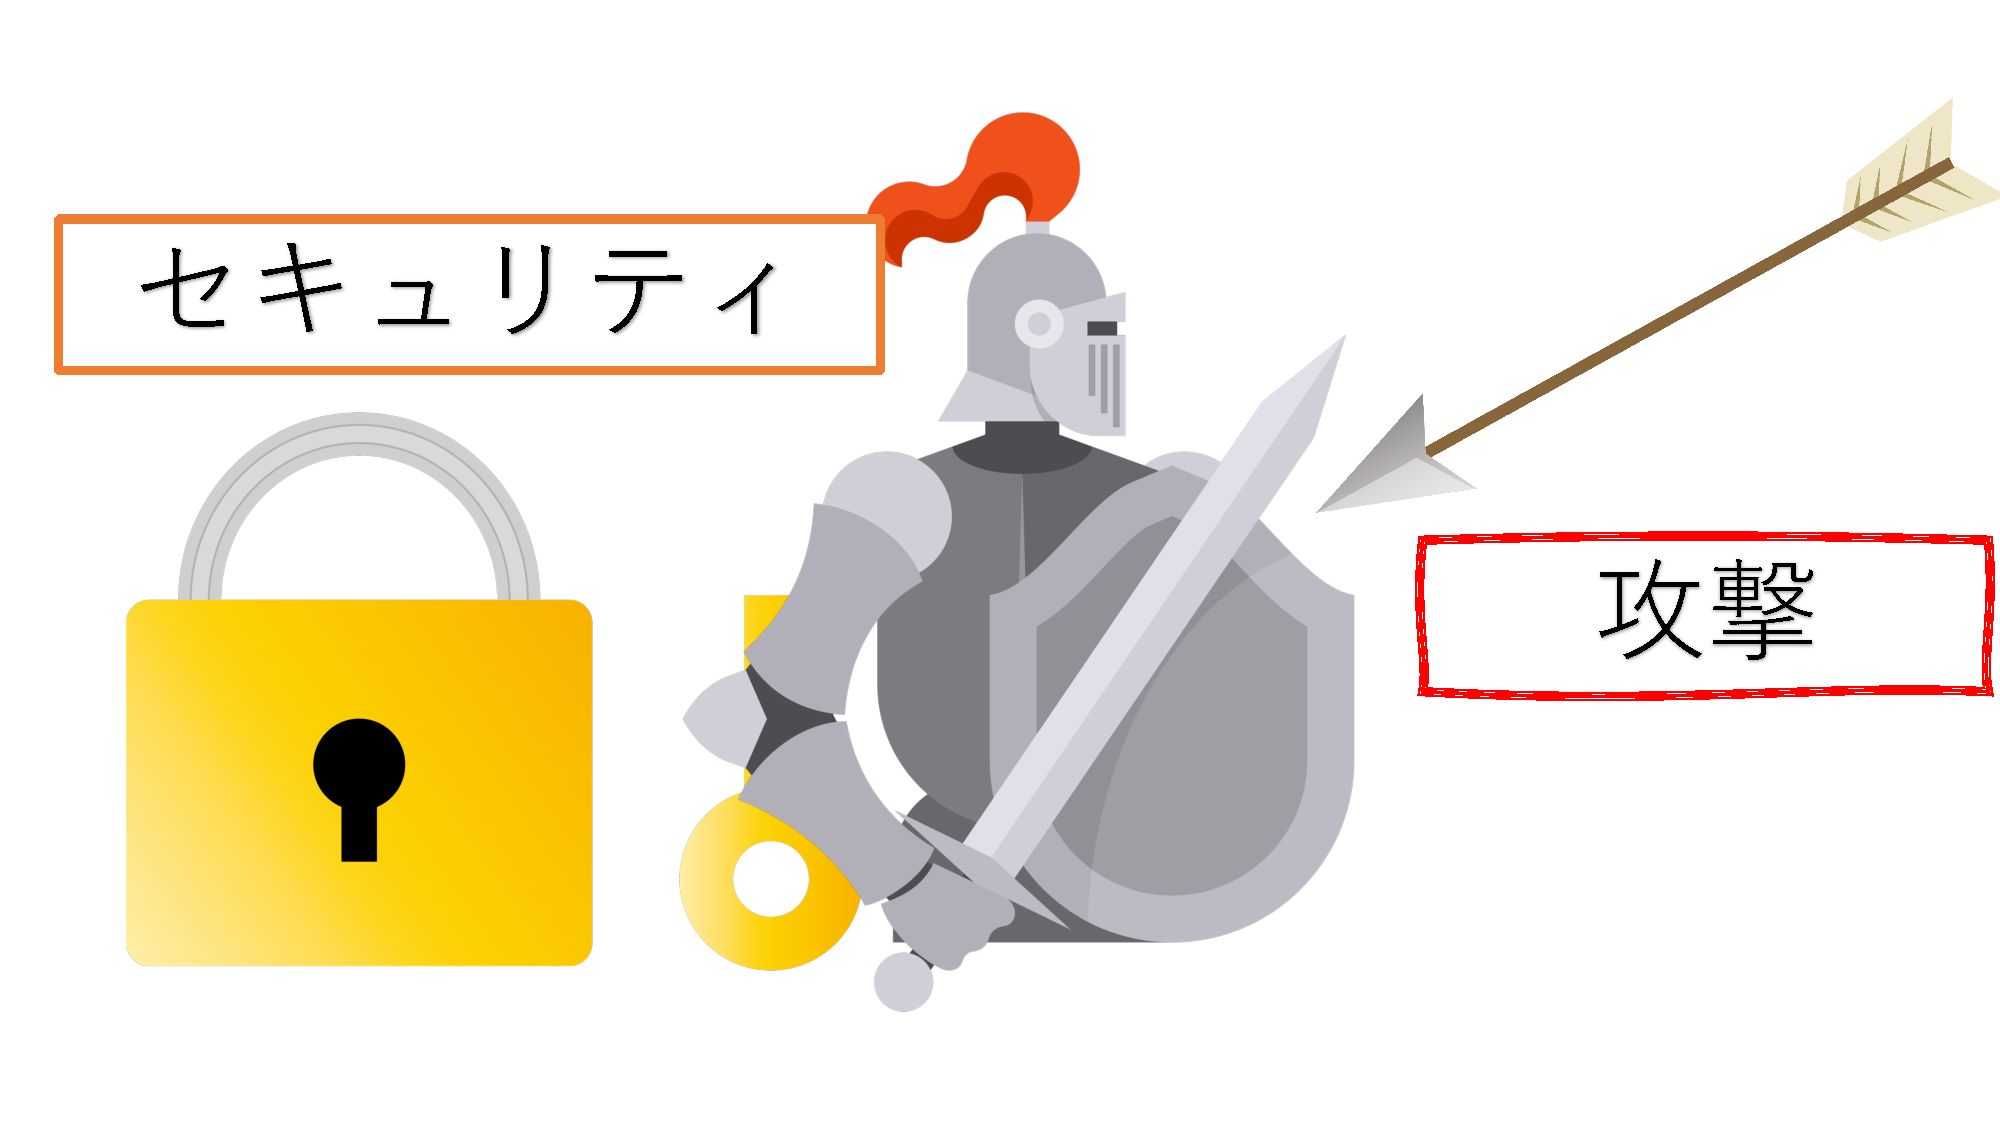
\includegraphics[width=7.000cm]{pswd_image_imp7.pdf}
              \newline
              Figure {\refstepcounter{Figure}\theFigure\label{seq:refFigure20}}:
              セキュリティ}
          \end{minipage}
        \end{figure}
        \item
        ショッピングサイトなどでは、ユーザー名とパスワードを利用して、さまざまな個人情報を管理しています。そのため、他人にユーザー名とパスワードを知られてしまうと、商品の購入履歴や住所、電話番号などの個人情報が漏洩することになります。
        \begin{figure}[h]
          \centering
          \begin{minipage}{5.228cm}
            {\upshape
              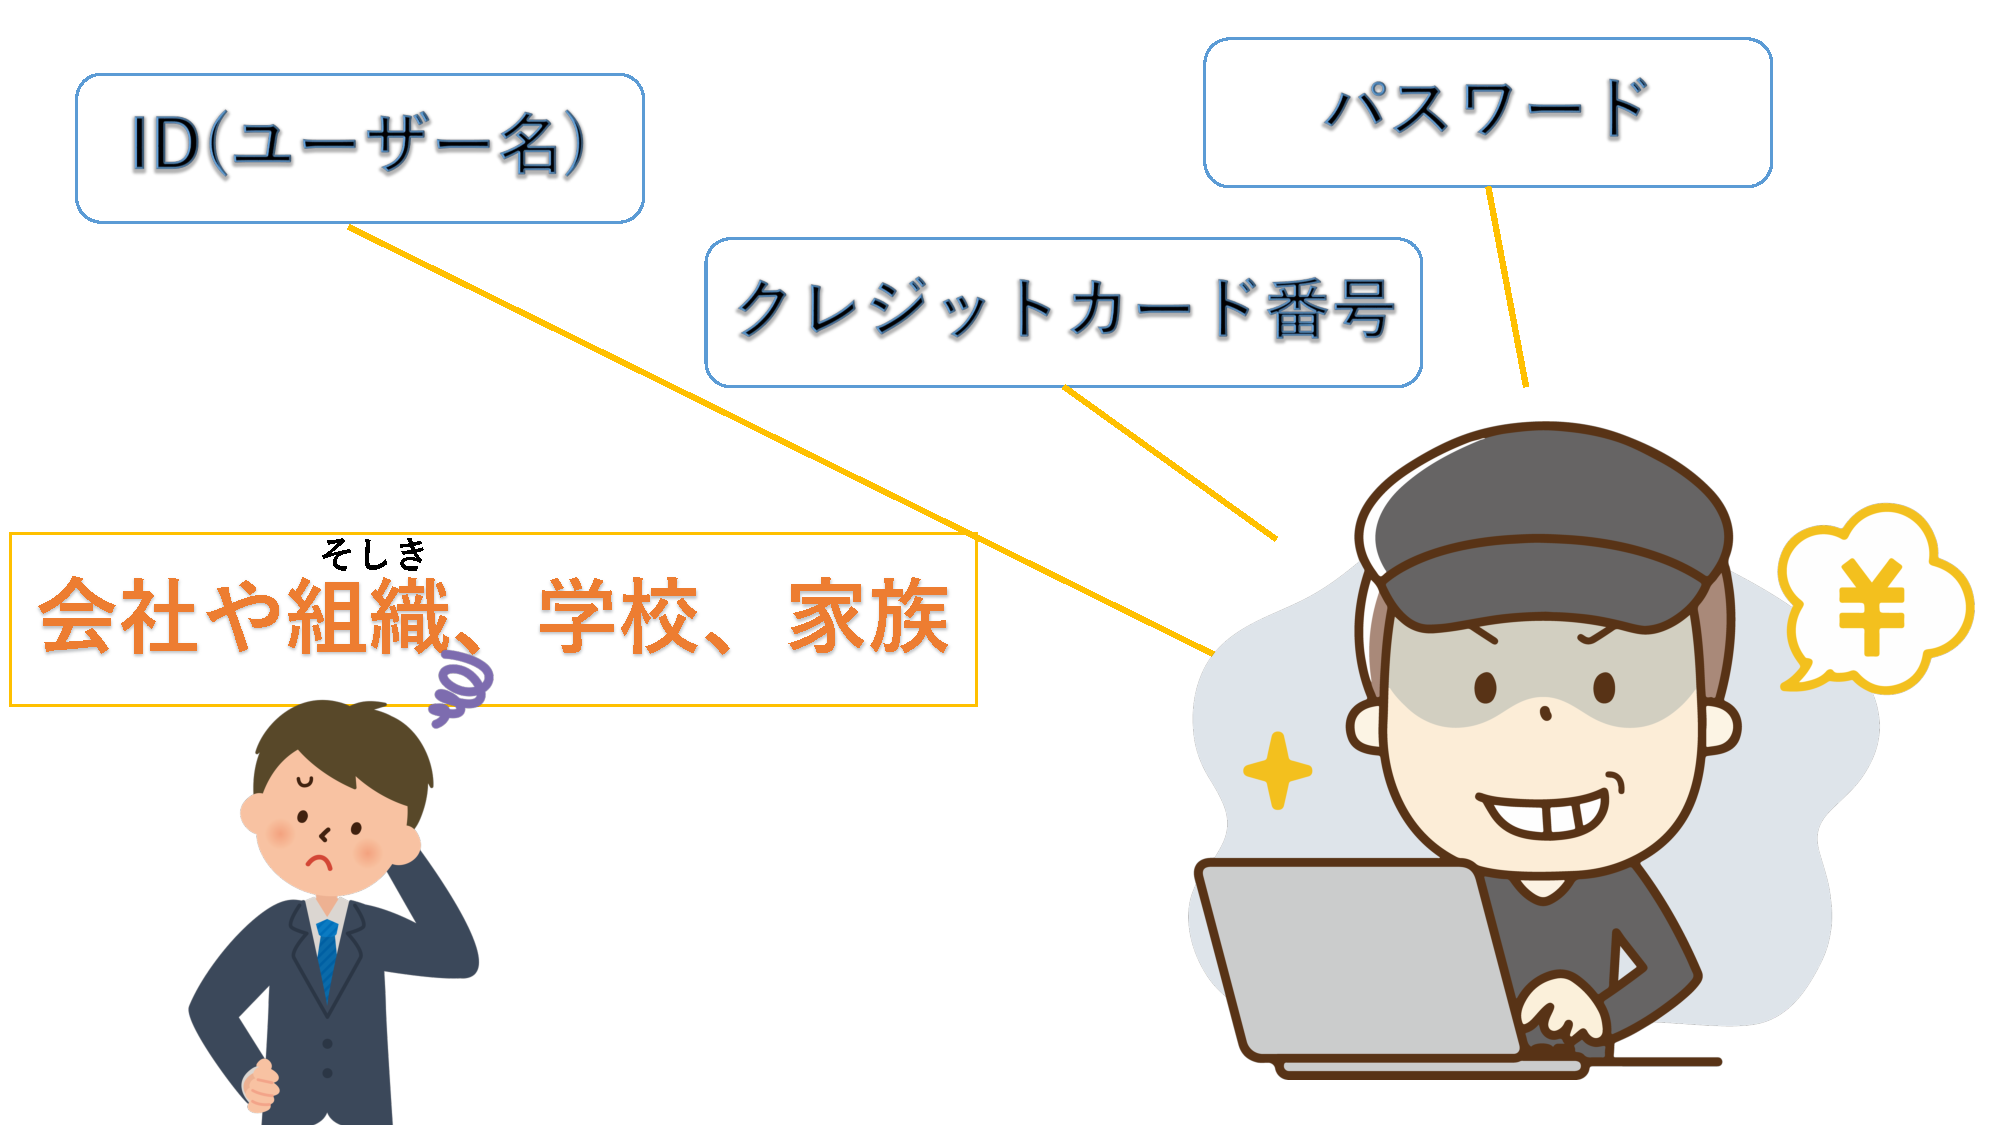
\includegraphics[width=7.000cm]{pswd_image_imp2.pdf}
              \newline
              Figure {\refstepcounter{Figure}\theFigure\label{seq:refFigure24}}:
              パスワード注意}
          \end{minipage}
        \end{figure}
        \item
        ショッピングサイトによっては、会員管理としてクレジットカード番号のデータを保存していることがあるため、自分の登録したクレジットカードで第三者に買い物をされてしまう危険性もあります。
        \begin{figure}[h]
          \centering
          \begin{minipage}{5.228cm}
            {\upshape
              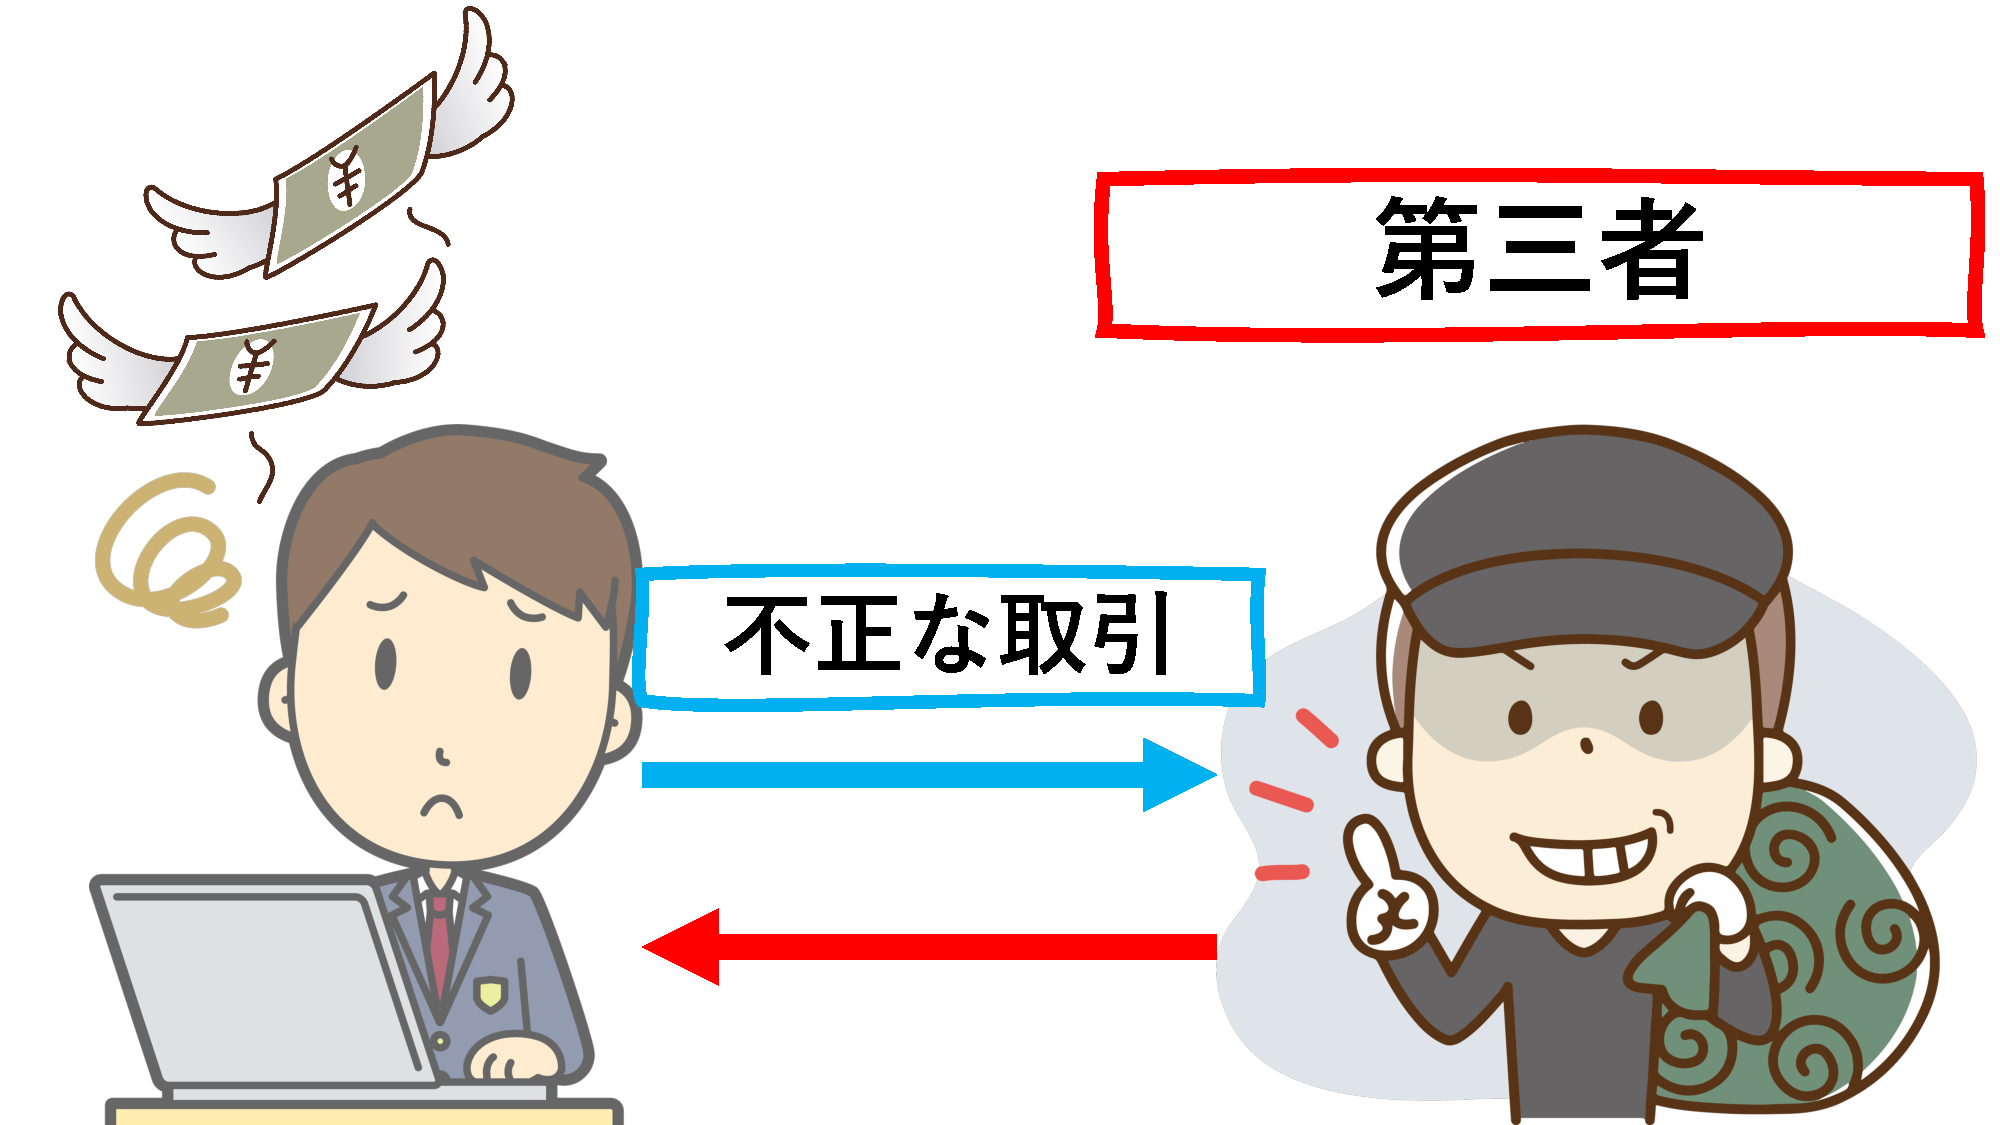
\includegraphics[width=7.000cm]{pswd_image_imp8.pdf}
              \newline
              Figure {\refstepcounter{Figure}\theFigure\label{seq:refFigure25}}:
              不正取引}
          \end{minipage}
        \end{figure}
        \item
              出典: 総務省『国民のための情報セキュリティサイト』\url{https://www.soumu.go.jp/main_sosiki/joho_tsusin/security_previous/kiso/k02_pass.htm}
        \end{itemize}
        \clearpage
  \item パスワードの制限について知ろう
        \begin{itemize}
          \item                                      
                次にユーザーを作成します。この図のようにFigure~\ref{seq:refFigure11}上から順にユーザー名、パスワード、再度入力用パスワードの入力の順になっています。またLinuxのユーザー名とパスワードの入力基準において以下の条件があります。
              
        
            \begin{figure}[h]
              \centering
              \begin{minipage}{5.228cm}
                {\upshape
                  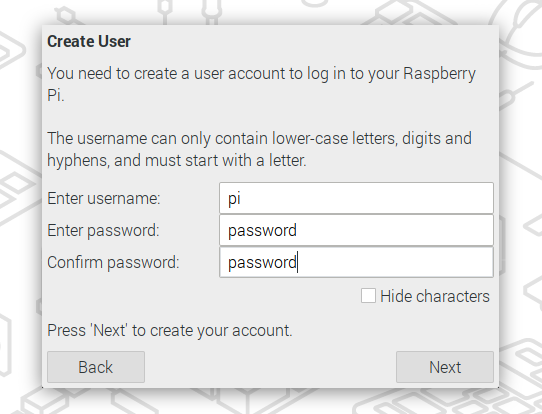
\includegraphics[width=7.000cm]{sw_image03.png}
                  \newline
                  Figure {\refstepcounter{Figure}\theFigure\label{seq:refFigure11}}:
                  ユーザー作成}
              \end{minipage}
            \end{figure}
          \end{itemize}

          \begin{itemize}
            \item
                  ユーザー名は小文字、数字、-、のみ使用可能。
            \item
                パスワードは8文字以上16文字以下。
            \item
                パスワードには以下の四つのカテゴリタイプの文字の内、三つのカテゴリタイプの文字を入れる必要がある。
          \end{itemize}
          \begin{table}[htbp]
            \centering
            \caption{文字タイプ表}
            \begin{tabular}{|c|c|}
            \hline
                タイプ & 実際に使用可能な文字 \\
                \hline
                大文字& ABCDEFGHIJKLMNOPQRSTUVWXYZ\\
                \hline
                小文字& abcdefghijklmnopqrstuvwxyz\\
                \hline
                数字 &0123456789\\
                \hline
                英数字以外の文字&~!@\#\$\%\textasciicircum\&*()\_+`\{\}\textbar[]\textbackslash:";'<>?,./\\
                \hline
            \end{tabular}
            \end{table}
            \begin{itemize}
              \item
                  注意事項
                  \begin{itemize}
                    \item
                        パスワードの先頭の大文字とパスワードの末尾の数字は、使用される文字クラスの数にはカウントされません。
                    \item
                    パスワードには辞書の単語やユーザーのログイン名を含めることはできません。
                    \item
                    文字を数字または英数字以外の文字に置き換えると、辞書の単語が受け入れられるようになります。(例)app1e, ta2ya
                    \item
                    自分が覚えやすいものになるべくしてください。※公になっている羅列やその他ですでに使用しているものは避けてください。
                  \end{itemize}
            \end{itemize}
    
\clearpage

    \item             
                知識を得たら実際にパスワードとユーザー名(ID)を決めよう
                \begin{itemize}
                  \item
                      \refstepcounter{Question}\theQuestion パスワードとユーザ名が決まったら下の記入欄に記入してみましょう。
                      \begin{table}[htbp]
                        \centering
                        
                        \begin{tabular}{|c|c|}
                        \hline
                            項目&この列を記入欄として扱ってください  \\
                            \hline
                            ユーザー名(ID)& \\
                            \hline
                            パスワード& \\
                            \hline
                        \end{tabular}
                        \end{table}
                  \item
                      記入が終わったら実際に入力してみます。その際にこのような画面Figure~\ref{seq:refFigure14}が出てきたらユーザー名(ID)かパスワードのどれかに不正な文字などが含まれている可能性があるのでもう一度確認しましょう。
                      \begin{figure}[h]
                        \centering
                        \begin{minipage}{5.228cm}
                          {\upshape
                            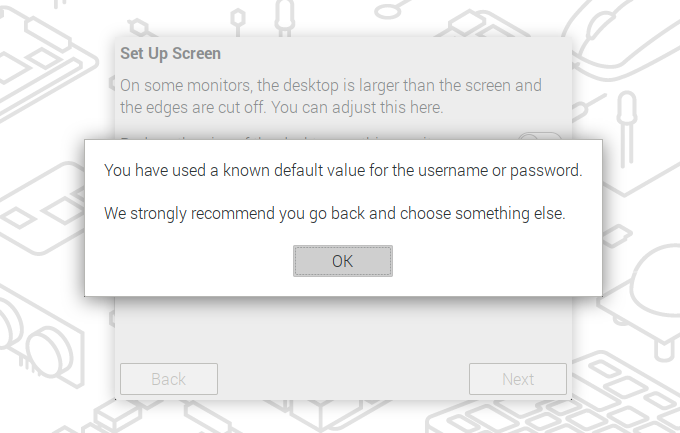
\includegraphics[width=7.000cm]{sw_image04.png}
                            \newline
                            Figure {\refstepcounter{Figure}\theFigure\label{seq:refFigure14}}:
                            エラー画面}
                        \end{minipage}
                      \end{figure}
                \end{itemize}
                \begin{itemize}
                  \item
                        次にスクリーンサイズを確認します。画面の大きさに対して表示されている解像度があっているか確認してください。TAの人と確認し、画面が歪んだりしていないか、縦横に伸びていないかを一緒に確認してください。問題の無い場合はNextを押して次に進みます。Figure~\ref{seq:refFigure15}
                        \begin{figure}[h]
                          \centering
                          \begin{minipage}{5.228cm}
                            {\upshape
                              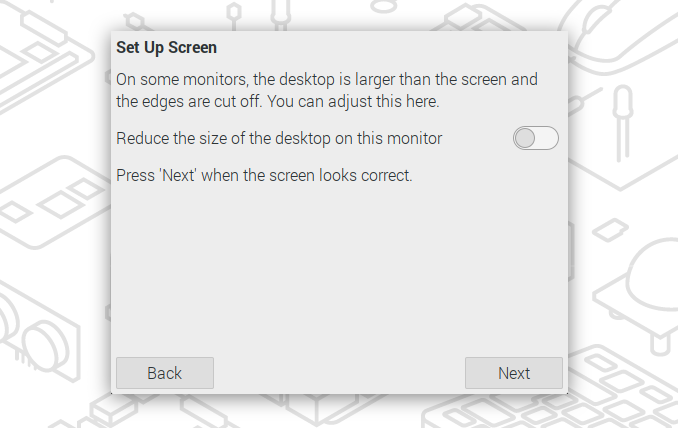
\includegraphics[width=7.000cm]{sw_image05.png}
                              \newline
                              Figure {\refstepcounter{Figure}\theFigure\label{seq:refFigure15}}:
                              スクリーンサイズ確認}
                          \end{minipage}
                        \end{figure}
                      \end{itemize}  
                      
  \clearpage                   
  \item     
        Wi-Fiを接続しよう
                \begin{itemize}
                  \item
                        次にWi-Fiの設定を行います。この赤枠の中に接続可能なWi-Fiの名前が表示されます。Figure~\ref{seq:refFigure16}
                        \item   
                        \refstepcounter{Question}\theQuestion またこのセクションではWi-FIのアドレスとパスワードが必要となるのでTA(ティーチングアシスタント(Teaching Assistant))の人からアドレスとパスワードを教えてもらい、下の欄に記入しておきましょう。    
                        \begin{table}[htbp]
                          \centering
                          
                          \begin{tabular}{|c|c|}
                          \hline
                              項目&この列を記入欄として扱ってください  \\
                              \hline
                              (例)Wi-Fiアドレス& ALGS630-12345678\\
                              \hline
                              (例)パスワード& 12345678910\\
                              \hline
                              Wi-Fiアドレス& \\
                              \hline
                              パスワード& \\
                              \hline
                          \end{tabular}
                          \end{table}
                        \item     
                        上部で記入したアドレスを選択してNextのボタンを押します。
                        \begin{figure}[h]
                          \centering
                          \begin{minipage}{5.228cm}
                            {\upshape
                              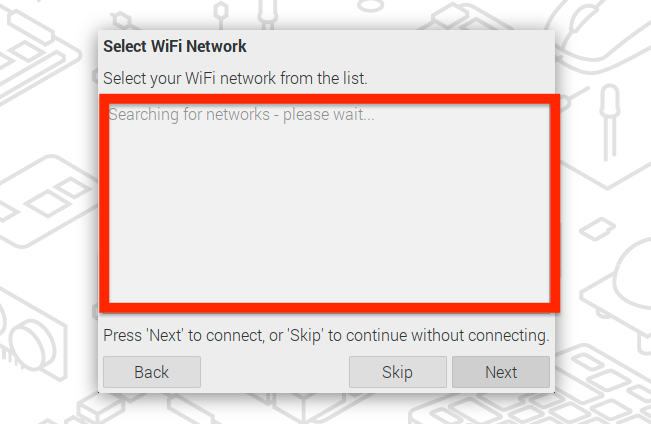
\includegraphics[width=7.000cm]{sw_image06kai.png}
                              \newline
                              Figure {\refstepcounter{Figure}\theFigure\label{seq:refFigure16}}:
                              Wi-Fi設定}
                          \end{minipage}
                        \end{figure}
                \end{itemize}
                \begin{itemize}
                  \item
                      そうするとパスワードを入力するように求められます。 ここでも上部で記入したパスワードを入力してNextを押します。
                      \begin{figure}[h]
                        \centering
                        \begin{minipage}{5.228cm}
                          {\upshape
                            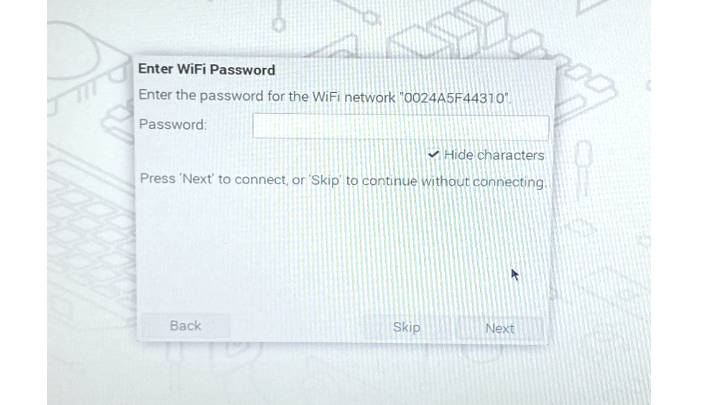
\includegraphics[width=10.000cm]{pswd_image_0404.png}
                            \newline
                            Figure {\refstepcounter{Figure}\theFigure\label{seq:refFigure17}}:
                            パスワード入力}
                        \end{minipage}
                      \end{figure}
                      
                \end{itemize}  
   \clearpage           
    \item
        アップデートの確認をしよう
                \begin{itemize}
                  \item
                      次の画面に進むとソフトウェアアップデートを求めらるので今回はアップデートをせずにSkipボタンを押して次の画面に遷移します。Figure~\ref{seq:refFigure18}
                      \begin{figure}[h]
                        \centering
                        \begin{minipage}{5.228cm}
                          {\upshape
                            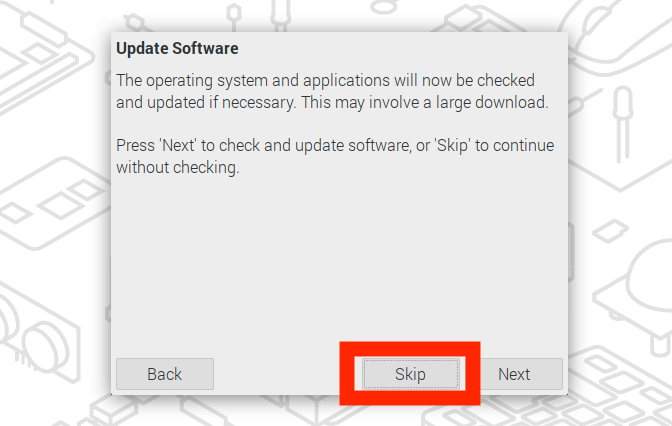
\includegraphics[width=7.000cm]{sw_image07.png}
                            \newline
                            Figure {\refstepcounter{Figure}\theFigure\label{seq:refFigure18}}:
                            ソフトウェアアップデート}
                        \end{minipage}
                      \end{figure}
                  \end{itemize}  
    \item
        再起動をしてraspberry piを始めよう
                \begin{itemize}
                  \item
                        次に大まかな初期設定が完了したので再起動を行います。画面右下にあるRestartのボタンを押してください。そうすると再起動が開始されます。
                        \begin{figure}[h]
                          \centering
                          \begin{minipage}{5.228cm}
                            {\upshape
                              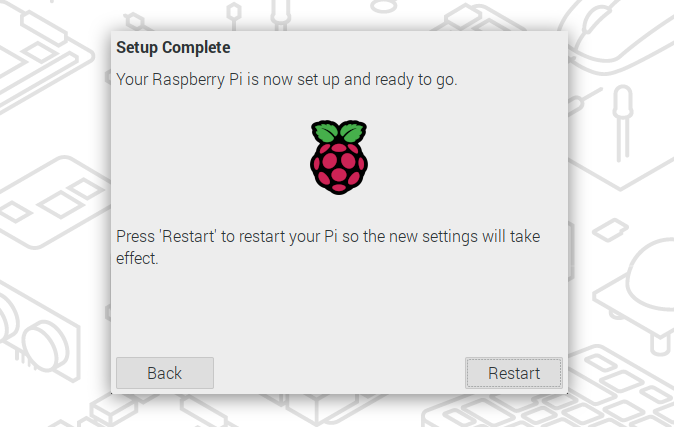
\includegraphics[width=7.000cm]{sw_image08.png}
                              \newline
                              Figure {\refstepcounter{Figure}\theFigure\label{seq:refFigure19}}:
                              再起動}
                          \end{minipage}
                        \end{figure}
                      \end{itemize}  
\clearpage                
\end{enumerate}

\end{document}